\chapter{Basis Functions}
\label{ch:dwt}
In Section \ref{sect:compression}, we introduced transform coding.
We said that any discrete signal $\bm v \in \mathbb{R}^M$ can be expressed in a different basis via a basis transform:
\begin{equation*}
  \bm v = \bm\Psi\bm w
\end{equation*}
where $\bm\Psi$ is the $M\times M$ basis matrix and $\bm w \in\mathbb{R}^M$ is the representation of $\bm v$ in the $\bm\Psi$ basis.

The particular classes of signals $\bm v$ that we are interested in are digital images and digital video.
The aim of this chapter is to construct a basis matrix $\bm\Psi$ that gives us a sparse representation of a wide range of such signals $\bm v$.

\section{Discrete Cosine Transform}
\label{sect:dct}
The first basis transform that we will describe is the Discrete Cosine Transform (DCT), one of the most widely used transforms in signal processing.
It underlies JPEG image compression and is used in various video compression algorithms such as MJPEG, MPEG, H.261 and H.263 \cite{zeng2013}.
\footnote{A related transform, known as the \emph{Modified DCT} is used in many lossy audio compression formats such as MP3, AAC and Vorbis.}

A DCT decomposes a signal in terms of cosine functions with different frequencies.
Its extensive use in lossy compression algorithms is due to the DCT's \emph{energy compaction} properties.
The majority of a transformed signal's energy is contained within relatively few coefficients - typically those corresponding to the lower frequency basis functions.

The DCT comes in a various versions that have minor differences between them.
In the following, we will describe the most widely used version, known as the \emph{DCT-II}, as well as its inverse transform, the \emph{DCT-III}.
We will refer to them simply as ``the DCT'' and ``the Inverse DCT'' (IDCT), respectively.

\subsection{One-Dimensional DCT}
Formally, the DCT $\bm w$ of a one-dimensional signal $\bm v$ of length $M$ is given by
\begin{equation}
  \label{eqn:dct_basis}
  w_k = c_k \sum_{n=1}^{M} v_n \, \cos\left(\frac{\pi(2n-1)(k-1)}{2M}\right) \qquad k = 1,\cdots,M
\end{equation}
where
\begin{equation*}
  c_k = \left\{\begin{array}{ll}
  \sqrt{\frac{1}{M}} & \qquad\mbox{if $k=1$}\\
  \sqrt{\frac{2}{M}} & \qquad\mbox{otherwise}\\
  \end{array}\right.
\end{equation*}
This transforms a signal $\bm v$ in the original domain (time or space) into its representation $\bm w$ in the DCT domain.

Conversely, given a signal $\bm w$ in the DCT domain, we can transform it back to the orignal (time or space) domain via the IDCT defined by
\begin{equation}
  \label{eqn:idct}
  v_n = \sum_{k=1}^M c_k w_k  \, \cos\left(\frac{\pi(2n-1)(k-1)}{2M}\right) \qquad n = 1,\cdots,M
\end{equation}

We can express equation (\ref{eqn:idct}) in the desired form $\bm v=\bm P\bm w$.
The entries of the basis matrix $\bm P$ are given by
\begin{equation}
  \label{eqn:idct_basis}
  P_{n,k} = c_k\, \cos\left(\frac{\pi(2n-1)(k-1)}{2M}\right).
\end{equation}
It can be verified that the basis matrix $\bm P$ is orthogonal, $\bm P^T\bm P=\bm I_M$.

\subsection{Multi-Dimensional DCT}
Once we know how to perform the DCT on a one-dimensional signal, we can easily extend the transform to multi-dimensional signals (images, video, etc).
To do so, we simply perform successive 1-D transforms along each dimension of the signal.
This is the \emph{seperability} of the DCT.

Suppose the signal of interest is a digital image.
That means that $\bm v$ is a $M_1\times M_2$ matrix where $M_1\times M_2$ is the resolution of the image.
To transform the signal, we first perform the DCT on every row of the matrix.
Following that, we perform the DCT on every column of the resulting matrix to get the final transformed signal.

\begin{figure}
  \centering
  \begin{subfigure}{0.45\textwidth}
    \centering
    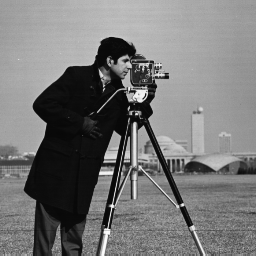
\includegraphics[width=\textwidth]{Chapter3/Images/cameraman.png}
    \caption{Original signal $\bm v$}
  \end{subfigure}
  \begin{subfigure}{0.45\textwidth}
    \centering
    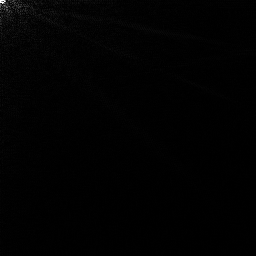
\includegraphics[width=\textwidth]{Chapter3/Images/dctCoeff.png}
    \caption{DCT of $\bm v$}
  \end{subfigure}
  \caption[Two-dimensional DCT applied to a digital image]{Panel (a) shows the original signal $\bm v$, a 256$\times$256 grayscale image known as ``cameraman''. Panel (b) illustrates the 2-D DCT of $\bm v$. The brightness of a an element increases with the absolute value of the corresponding DCT coefficient. (The high-frequency coefficients have been enhanced to show more detail).}
  \label{fig:ch3:dct}
\end{figure}

Figure \ref{fig:ch3:dct} shows an example of a 2-D signal $\bm v$ and its transform $\bm w$.
Note that the majority of the energy of the transformed signal is concentrated in the top left corner.
Most of the DCT coefficients are zero or very close to zero.

\begin{figure}
  \centering
  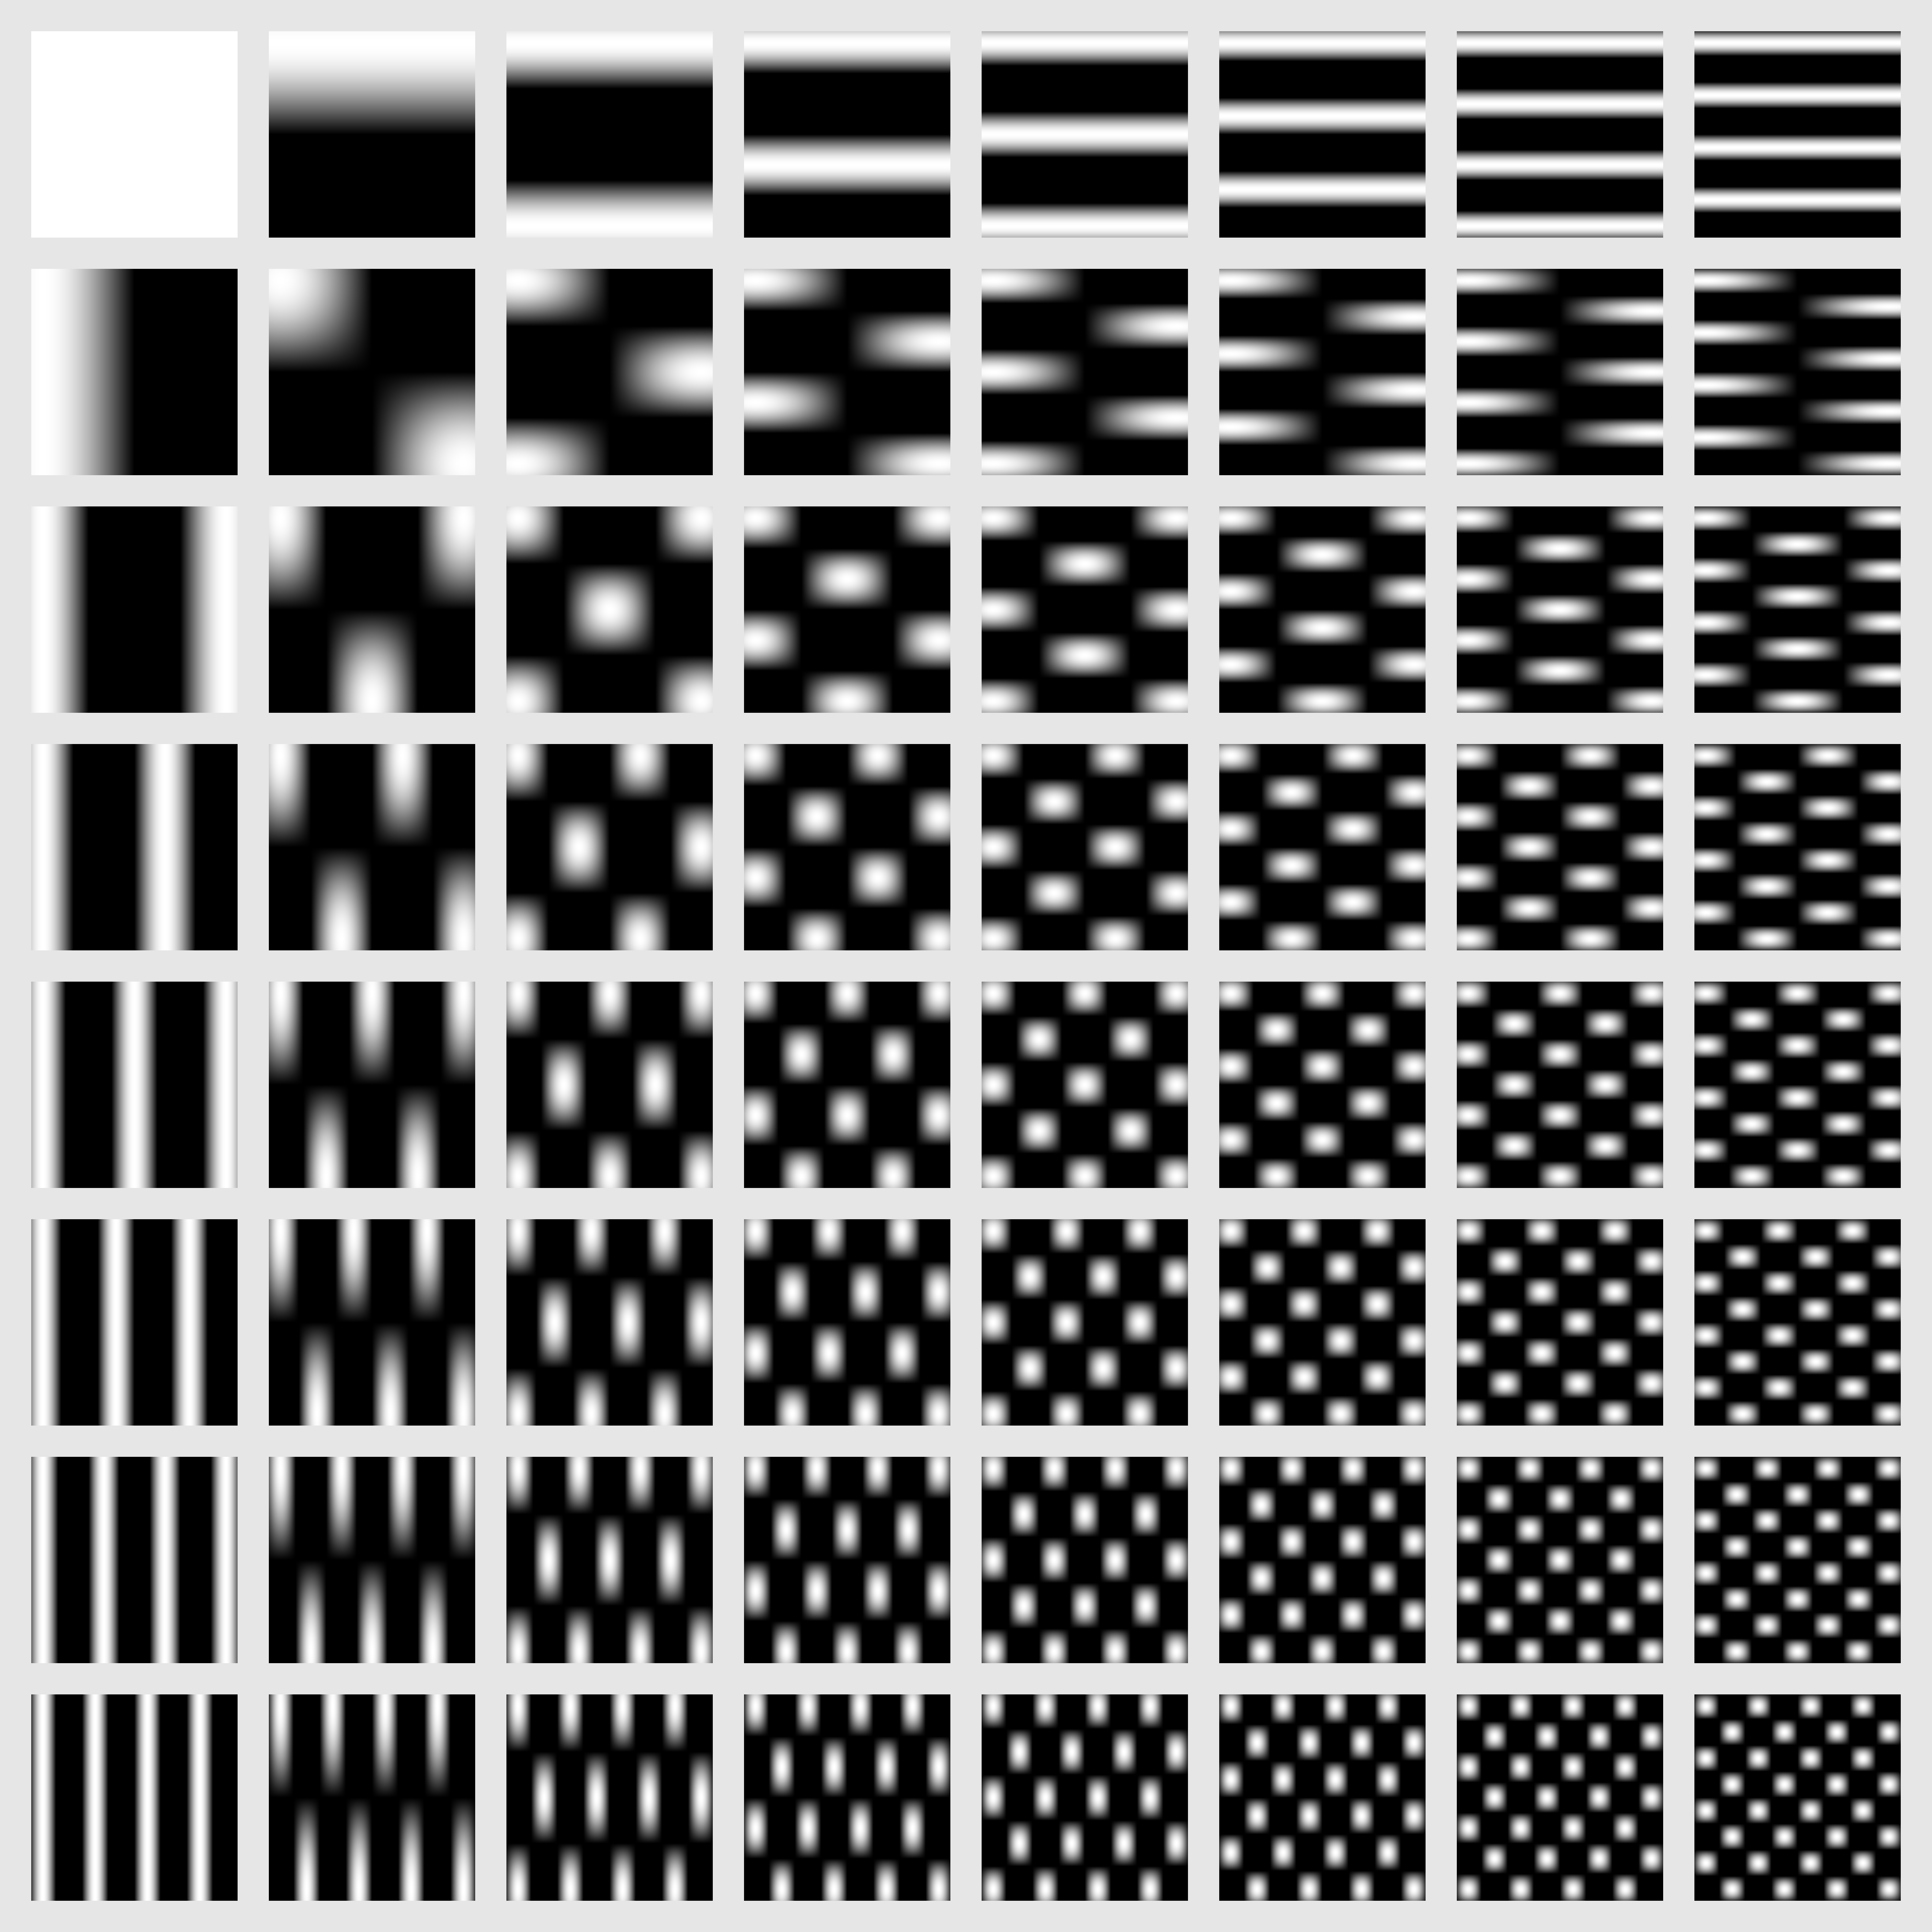
\includegraphics[width=0.5\textwidth]{Chapter3/Images/dct2functions.png}
  \caption[The 2-D DCT basis functions]{The 2-D DCT basis functions that are used by the DCT to decompose a $4\times 4$ image. 
    The spatial frequency increases towards the bottom right corner.}
  \label{fig:2D-DCT}
\end{figure}

In Figure \ref{fig:2D-DCT}, we show the 2-D basis functions that would used by the DCT to decompose a signal of size $4\times 4$.
Each basis function is characterised by a horizontal and vertical spatial frequency.
Typically, natural images are mostly made up of low-frequency components and the corresponding coefficients are therefore relatively large.
The highest-frequency components are usually only needed to describe very fine details.

To compute the DCT of a video, we first compute the 2-D DCT for each individual frame of the video followed by a 1-D DCT across the temporal axis for each pixel.
The DCT basis functions in 3-D are characterised by a horizontal and vertical spatial frequency, as well as an additional temporal frequency component.

For a discussion on the properties of the DCT, see \cite{khayam2003}

\section{Discrete Wavelet Transform}
Wavelets have become a very popular tool in signal processing.
Their energy compaction properties are on par and often superior to those of the DCT for a wide range of signal classes.
Moreover, the multiresolution properties of wavelets allow us to analyze signals at different scales.

In 2000, the JPEG committee released a new image coding standard, JPEG2000, that is gradually replacing the original JPEG standard.
The new format moved away from the DCT and uses a Discrete Wavelet Transform (DWT) instead \cite{usevitch2001}.

The aim of the following sections is to provide some intuition on the general properties of wavelets.
We will discuss how a wavelet basis can be constructed at multiple resolution levels and how the DWT can be computed in practice.
We will refrain from going to deep into mathematical detail and instead direct the interested reader to \cite{mallat1999,daubechies1992}.

\subsection{Introduction to Wavelets}
To motivate wavelets, consider again the one-dimensional signal $\bm v$ of length $M$.
Suppose, for simplicity, that $M$ is a power of $2$, $M = 2^q$ say.
We can view $\bm v$ as a piecewise-constant function $v(x)$ on the half-open interval $[0,1)$, where $v(x) = v_i$ if $x \in [\frac{i-1}{M}, \frac{i}{M})$.

Let $V^j$ denote the vector space containing all piecewise-constant functions $f$ defined on the interval $[0,1)$ that consist of $2^j$ pieces, each of which is constant across a sub-interval of size $2^{-j}$.
Thus, $V^0$ consists of all functions that are constant on $[0,1)$, while $V^1$ consists of all functions that have two constant pieces, one over $[0,1/2)$ and one over $[1/2,1)$.
In particular, our signal $v(x)$ resides in the space $V^q$.

Note that if $f \in V^j$, then $f \in V^{j+1}$.
Thus, the vector spaces $V^j$ are nested: $V^0 \subset V^1 \subset V^2 \subset \cdots$.

We need to choose a basis for each vector space $V^j$.
To do so, we introduce a \emph{scaling function} (also known as \emph{scalet}, or \emph{father wavelet}) that is usually denoted $\phi(x)$.
The form of the scaling function depends on the particular choice of wavelet decomposition.

\begin{figure}
  \centering
  \begin{subfigure}{0.4\textwidth}
    \centering
    \begin{tikzpicture}[xscale=2]
      \draw [thin,->] (0,-1.5) -- (0,1.5);
      \draw [thin,->] (-0.5,0) -- (1.5,0) node[below]{\small$x$};
      \draw [very thick] (-0.2,0) -- (0,0) node[below left]{\small$0$} -- (0,1) node[left]{\small$1$} -- (1,1) -- (1,0) node[below]{\small$1$} -- (1.3,0);
    \end{tikzpicture}
    \caption{Haar scaling function $\phi(x)$}
    \label{fig:haar_scaling}
  \end{subfigure}
  \begin{subfigure}{0.4\textwidth}
    \centering
    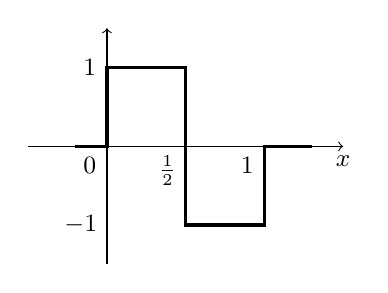
\begin{tikzpicture}[xscale=2]
      \draw [thin,->] (0,-1.5) -- (0,1.5);
      \draw [thin,->] (-0.5,0) -- (1.5,0) node[below]{\small$x$};
      \draw [very thick] (-0.2,0) -- (0,0) node[below left]{\small$0$} -- (0,1) node[left]{\small $1$} -- (0.5,1) -- (0.5,-1) -- (1,-1) -- (1,0) node[below left]{\small $1$} -- (1.3,0);
      \node at (0,-1)[left]{\small$-1$};
      \node at (0.5,0)[below left]{\small $\frac{1}{2}$};
    \end{tikzpicture}
    \caption{Haar mother wavelet $\psi(x)$}
    \label{fig:haar_mother}
  \end{subfigure}
  \caption{The scaling function and wavelet function for the Haar wavelets.}
  \label{fig:haar_1d}
\end{figure}

For example, for the \emph{Haar wavelets}, the scaling function is given by
\begin{equation}
  \label{eqn:haar_scale}
  \phi(x) = \left\{ \begin{array}{rl}
    1& \qquad \mbox{if $0\leq x < 1$}\\
    0& \qquad \mbox{otherwise}
  \end{array}\right.
\end{equation}
See Figure \ref{fig:haar_scaling} for a plot of $\phi(x)$.

Given the scaling function $\phi(x)$, we can define the following basis for $V^j$:
\begin{equation}
  \label{eqn:haar_scaling_basis}
  \phi_k^j(x) := 2^{j/2}\phi(2^j x-k) \qquad k = 0,\cdots, 2^j-1
\end{equation}

Using this basis, we can decompose our signal $v(x)\in V^q$ as 
\begin{equation*}
  v(x) = \sum_{k=0}^{2^q-1} c_k^q \phi_k^q(x)
\end{equation*}
For the particular scaling function defined in equation (\ref{eqn:haar_scale}), we can see that $c_k^q = v_{k+1}$.

To obtain \emph{wavelets}, consider the \emph{orthogonal complement} of $V^j$ in $V^{j+1}$ and denote it $W^j$. 
That is, $W^j = \{f \in V^{j+1} :\, \langle f,g\rangle = 0\,\, \forall g \in V^j\}$ where the inner product $\langle f,g\rangle$ is defined by
\begin{equation*}
  \langle f,g\rangle = \int_0^1f(x)g(x)dx.
\end{equation*}
By forming a basis for $W^j$, we obtain a set of \emph{wavelet functions} $\{\psi_k^j,\, k=0,\cdots,2^j-1\}$.
Wavelet functions can be constructed by scaling and shifting a so-called \emph{mother wavelet} $\psi(x)$ as follows:
\begin{equation}
  \label{eqn:haar_wavelet_basis}
  \psi_k^j(x) = 2^{j/2}\psi(2^j x - k) \qquad k = 0,\cdots, 2^j-1
\end{equation}

For the Haar wavelets, the mother wavelet is given by:
\begin{equation}
\label{eqn:haar_mother}
  \psi(x) = \left\{\begin{array}{rl}
  1&\qquad 0 \leq x < 1/2\\
  -1&\qquad 1/2 \leq x < 1\\
  0&\qquad\mbox{otherwise}
  \end{array}\right.
\end{equation}
The Haar mother wavelet is shown in Figure \ref{fig:haar_mother}.

Note that, since the scaling functions $\phi_k^j$ form a basis of $V^j$ and the wavelet functions $\psi_k^j$ form a basis of $W^j$, and since $W^j$ is the orthogonal complement to $V^j$ in $V^{j+1}$, it follows that the set $\{\phi_k^j, \psi_k^j: k=0,\cdots,2^j-1\}$ forms a basis of the vector space $V^{j+1}$.

This allows us to express our signal $v \in V^q$ as 
\begin{equation*}
  v(x) = \sum_{k=0}^{2^{q-1}-1} d_k^{q-1}\psi_k^{q-1}(x) + \sum_{k=0}^{2^{q-1}-1} c_k^{q-1}\phi_k^{q-1}(x)
\end{equation*}
This gives us the first level of the discrete wavelet transform of $v$.
The coefficients $c_k$ and $d_k$ are sometimes referred to as ``approximation'' coefficients and ``detail'' coefficients, respectively.

We can continue the decomposition by splitting the basis for $V^{q-1}$ into the bases for $V^{q-2}$ and $W^{q-2}$ to get the next level of the transform:
\begin{equation*}
  v(x) = \sum_{k=0}^{2^{q-1}-1} d_k^{q-1}\psi_k^{q-1}(x) + \sum_{k=0}^{2^{q-2}-1} d_k^{q-2}\psi_k^{q-2}(x) + \sum_{k=0}^{2^{q-2}-1} c_k^{q-2}\phi_k^{q-2}(x)
\end{equation*}
To get the full decomposition, we continue in this fashion up to the $q$th level:
\begin{equation*}
  v(x) = \sum_{j=0}^{q-1} \sum_{k=0}^{2^j-1} d_k^{j} \psi_k^j(x) + c_0^0\phi(x)
\end{equation*}
The full Discrete Wavelet Transform of $\bm v$ consists of the coefficients
\begin{equation*}
  \{c_0^0, d_k^j:\,j=0,\cdots,q-1, \, k=0,\cdots,2^j-1\}.
\end{equation*}


\subsection{Computing the DWT}

\begin{figure}
  \centering
  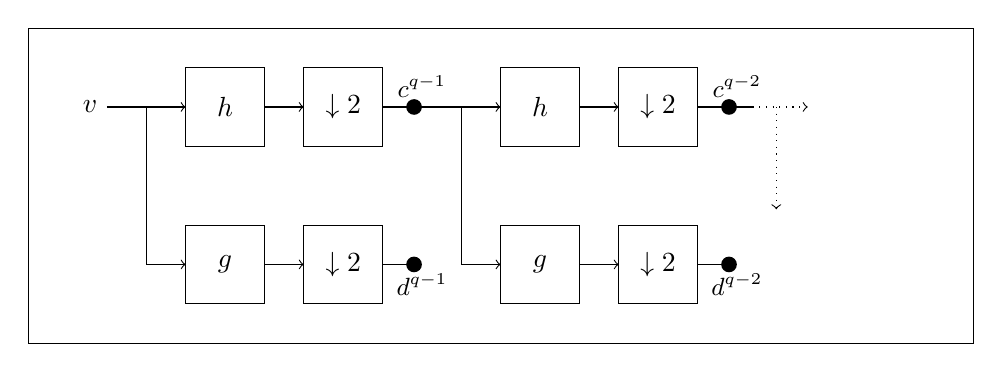
\begin{tikzpicture}
    \draw (0,0) rectangle (12,4);
    \draw (1,3) node[left]{$v$} -- (1.5,3);
    \draw (1.5,1) -- (1.5,3);
    \draw [->](1.5,3) -- (2,3);
    \draw [->](1.5,1) -- (2,1);
    \draw (2,2.5) rectangle (3,3.5);
    \node at (2.5,3) {$h$};
    \draw (2,0.5) rectangle (3,1.5);
    \node at (2.5,1) {$g$};
    \draw [->](3,1) -- (3.5,1);
    \draw (3.5,0.5) rectangle (4.5,1.5);
    \node at (4,1) {$\downarrow 2$};
    \draw (4.5,1) -- (5,1) node [below] {\small$d^{q-1}$};
    \node at (4.9,1)[shape=circle, fill=black, inner sep=2pt, minimum size=2pt] {};
    \draw [->](3,3) -- (3.5,3);
    \draw (3.5,2.5) rectangle (4.5,3.5);
    \node at (4,3) {$\downarrow 2$};
    \draw [->](4.5,3) -- (6,3);
    \draw [->](5.5,3) -- (5.5,1) -- (6,1);
    \node at (5,3) [above] {\small$c^{q-1}$};
    \node at (4.9,3) [shape=circle, fill=black, inner sep=2pt, minimum size=2pt] {};
    \draw (6,2.5) rectangle (7,3.5);
    \node at (6.5,3){$h$};
    \draw (6,0.5) rectangle (7,1.5);    
    \node at (6.5,1){$g$};
    \draw [->] (7,3) -- (7.5,3);
    \draw (7.5,2.5) rectangle (8.5,3.5);
    \node at (8,3) {$\downarrow 2$};
    \draw [->] (7,1) -- (7.5,1);
    \draw (7.5,0.5) rectangle (8.5,1.5);
    \node at (8,1) {$\downarrow 2$};
    \draw (8.5,1) -- (9,1) node [below] {\small$d^{q-2}$};
    \node at (8.9,1) [shape=circle, fill=black, inner sep=2pt, minimum size=2pt] {};
    \draw (8.5,3) -- (9.2,3);
    \draw [->,dotted](9.2,3) -- (9.9,3);
    \draw [->,dotted](9.5,3) -- (9.5,1.7);
    \node at (8.9,3) [shape=circle, fill=black, inner sep=2pt, minimum size=2pt] {};
    \node at (9,3) [above] {\small$c^{q-2}$};
  \end{tikzpicture}
  \caption[Filter Bank computation of the DWT]{The first two levels of the DWT of the signal $\bm v$ of length $2^q$ via a filter bank.}
  \label{fig:filterbank}
\end{figure}

In practice, we can compute one level of the DWT coefficients by passing the signal $v$ through a \emph{low-pass filter} $h$ and a high-pass filter $g$, respectively, and then downsampling the results by a factor of two.
Passing $v$ through the filters $h$ and $g$ results in the \emph{convolutions}:
\begin{equation*}
  \begin{split}
    (v\star h)(x) &:= \sum_{k=-\infty}^\infty v(k)h(x-k)\\
    (v\star g)(x) &:= \sum_{k=-\infty}^\infty v(k)g(x-k)
  \end{split}
\end{equation*}
To downsample by a factor of two, we remove every second sample:
\begin{equation*}
  (v\downarrow 2)(x) := v(2x)
\end{equation*}

Overall, these computations can be performed by multiplying the vector $\bm v$ by a matrix $\bm H$ and a matrix $\bm G$ to get the approximation and detail coefficients, respectively.

To compute the next stage, we take the approximation coefficients of the current stage and pass them again through the filter bank.
The procedure is depicted in Figure \ref{fig:filterbank}.

The coefficients of the filters $h(x)$ and $g(x)$ depend on our choice of the scaling function $\phi(x)$ and mother wavelet function $\psi(x)$ and must satisfy the relations
\begin{equation*}
  \begin{split}
    \phi(x) &= \sqrt{2}\sum_{k=-\infty}^\infty h(k)\phi(2x - k)\\
    \psi(x) &= \sqrt{2}\sum_{k=-\infty}^\infty g(k)\phi(2x - k)
  \end{split}
\end{equation*}
as well as
\begin{equation*}
  g(k) = (-1)^k h(1-k).
\end{equation*}

For the Haar wavelets (\ref{eqn:haar_scale},\ref{eqn:haar_mother}), the filter coefficients are
\begin{equation*}
  \begin{split}
    h(0) = h(1) &= \frac{1}{\sqrt{2}}, \qquad h(k) = 0 \mbox{  if $k\neq 0,1$}\\
    g(0) = -g(1) &= \frac{1}{\sqrt{2}}, \qquad g(k) = 0 \mbox{  if $k\neq 0,1$}
  \end{split}
\end{equation*}

The approximation coefficients for the first stage of the Haar DWT of signal $\bm v \in\mathbb{R}^M$, with $M=2^q$, are thus given by $\bm H^q \bm v$ where $\bm H^q$ is the $2^{q-1}\times 2^q$ matrix defined by
\begin{equation}
  \label{eqn:haar_H}
  \bm H^q_{haar} = \frac{1}{\sqrt{2}} \begin{bmatrix}
    1&1&0&0&\cdots&0&0\\
    0&0&1&1&\cdots&0&0\\
    \vdots&\vdots&\vdots&\vdots&\ddots&\vdots&\vdots\\
    0&0&0&0&\cdots&1&1
  \end{bmatrix}
\end{equation}
To get the corresponding detail coefficients, we multiply $\bm v$ by the $2^{q-1}\times 2^q$ matrix $\bm G^q$ defined by
\begin{equation}
  \label{eqn:haar_G}
  \bm G^q_{haar} = \frac{1}{\sqrt{2}} \begin{bmatrix}
    1&-1&0&0&\cdots&0&0\\
    0&0&1&-1&\cdots&0&0\\
    \vdots&\vdots&\vdots&\vdots&\ddots&\vdots&\vdots\\
    0&0&0&0&\cdots&1&-1
  \end{bmatrix}
\end{equation}

Overall, to perform the discrete Haar wavelet transform at the first scale, we multiply $\bm v$ by
\begin{equation*}
  \bm P^{(1)}_{haar} = \begin{bmatrix}
    \bm H^q \\
    \bm G^q \\
  \end{bmatrix}
\end{equation*}
where we dropped the $haar$-subscript on $\bm H$ and $\bm G$ for ease of viewing.

To compute the transform at the second scale, we replace $\bm H^q$ by $\bm H^{q-1}\bm H^q$ and $\bm G^{q-1}\bm h^q$:
\begin{equation*}
  \bm P^{(2)}_{haar} = \begin{bmatrix}
    \bm H^{q-1} \bm H^q \\
    \bm G^{q-1} \bm H^q \\
    \bm G^q \\
  \end{bmatrix}
\end{equation*}

We can continue this process until the $q$th scale to get the full Haar wavelet transform matrix:
\begin{equation*}
  \bm P^{(q)}_{haar} = \begin{bmatrix}
    \bm H^1 \bm H^2 \cdots \bm H^{q-1} \bm H^q \\
    \bm G^1 \bm H^2 \cdots \bm H^{q-1} \bm H^q \\
    \vdots\\
    \bm G^{q-2} \bm H^{q-1} \bm H^q \\
    \bm G^{q-1} \bm H^q \\
    \bm G^q \\
  \end{bmatrix}
\end{equation*}
Note that the size of the transform matrix $\bm P^j_{haar}$ is $M\times M$ and is not affected by the scale $j$.

To form the basis matrix $\bm\Psi$ such that $\bm v = \bm\Psi\bm w$ corresponding to the DWT at scale $j$, we can invert the matrix $\bm P^{(j)}_{haar}$:
\begin{equation}
  \label{eqn:dwt_basis}
  \bm\Psi = \left(\bm P^{(j)}_{haar}\right)^{-1}
\end{equation}
In practice, it is desirable to work with orthonormal wavelet bases because they lead to orthogonal transform matrices, so that $\left(\bm P^{(j)}\right)^{-1}=\left(\bm P^{(j)}\right)^T$.
This orthoganility property is provided by Haar wavelets.
Therefore, the basis matrix $\bm\Psi$ from equation (\ref{eqn:dwt_basis}) can also be obtained as follows:
\begin{equation}
  \label{eqn:haar1_basis}
  \bm\Psi = \left(\bm P^{(j)}_{haar}\right)^T.
\end{equation}


\subsection{Two-Dimensional Haar Wavelets}
In Figure \ref{fig:haar_1d}, we showed the 1-dimensional Haar scaling function $\phi(x)$ and wavelet function $\psi(x)$.
In general, we can define the 2-dimensional scaling wavelet functions by taking the products of their one-dimensional versions:
\begin{equation}
\label{eqn:2d_haar_wavelets}
  \begin{split}
    \phi(x,y) &= \phi(x) \phi(y)\\
    \psi^H(x,y) &= \phi(x) \psi(y) \\
    \psi^V(x,y) &= \psi(x) \phi(y) \\
    \psi^D(x,y) &= \psi(x) \psi(y)
  \end{split}
\end{equation}

\begin{figure}
\centering
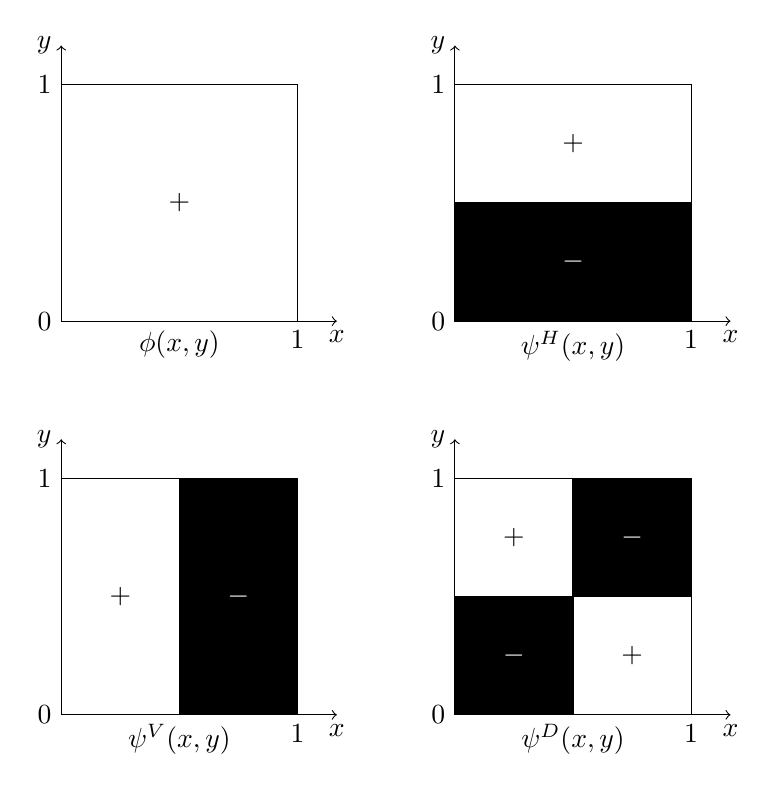
\begin{tikzpicture}
  \draw (0,5) rectangle (3,8);
  \draw (5,5) rectangle (8,8);
  \draw (0,0) rectangle (3,3);
  \draw (5,0) rectangle (8,3);

  \draw [<->] (0,8.5) -- (0,5) -- (3.5,5);
  \draw [<->] (5,8.5) -- (5,5) -- (8.5,5);
  \draw [<->] (0,3.5) -- (0,0) -- (3.5,0);
  \draw [<->] (5,3.5) -- (5,0) -- (8.5,0);

  \node at (1.5,5) [below] {$\phi(x,y)$};
  \node at (0,5) [left] {$0$};
  \node at (0,8) [left] {$1$};
  \node at (3,5) [below] {$1$};
  \node at (3.5,5) [below] {$x$};
  \node at (0,8.5) [left] {$y$};

  \node at (6.5,5) [below] {$\psi^H(x,y)$};
  \node at (5,5) [left] {$0$};
  \node at (5,8) [left] {$1$};
  \node at (8,5) [below] {$1$};
  \node at (8.5,5) [below] {$x$};
  \node at (5,8.5) [left] {$y$};

  \node at (1.5,0) [below] {$\psi^V(x,y)$};
  \node at (0,0) [left] {$0$};
  \node at (0,3) [left] {$1$};
  \node at (3,0) [below] {$1$};
  \node at (3.5,0) [below] {$x$};
  \node at (0,3.5) [left] {$y$};

  \node at (6.5,0) [below] {$\psi^D(x,y)$};
  \node at (5,0) [left] {$0$};
  \node at (5,3) [left] {$1$};
  \node at (8,0) [below] {$1$};
  \node at (8.5,0) [below] {$x$};
  \node at (5,3.5) [left] {$y$};

  \draw [fill=black] (5,5) rectangle (8,6.5);
  \draw [fill=black] (1.5,0) rectangle (3,3);
  \draw [fill=black] (5,0) rectangle (6.5,1.5);
  \draw [fill=black] (6.5,1.5) rectangle (8,3);

  \node at (1.5,6.5){$\bm +$};  
  % \node at (0.75,5.75){$\bm +$};
  % \node at (2.25,5.75){$\bm +$};
  % \node at (0.75,7.25){$\bm +$};
  % \node at (2.25,7.25){$\bm +$};
  % \draw (1.5,5) -- (1.5,8);
  % \draw (0,6.5) -- (3,6.5);

 \node at (6.5,7.25){$\bm +$};
 \node at (6.5,5.75){\textcolor{white}{$\bm -$}};
  % \node at (5.75,5.75){\textcolor{white}{$\bm -$}};
  % \node at (7.25,5.75){\textcolor{white}{$\bm -$}};
  % \node at (5.75,7.25){$\bm +$};
  % \node at (7.25,7.25){$\bm +$};
  % \draw (6.5,5) -- (6.5,8);
  % \draw (5,6.5) -- (8,6.5);


  \node at (0.75,1.5){$\bm +$};
  \node at (2.25,1.5){\textcolor{white}{$\bm -$}};

  \node at (5.75,2.25){$\bm +$};
  \node at (7.25,0.75){$\bm +$};
  \node at (5.75,0.75){\textcolor{white}{$\bm -$}};
  \node at (7.25,2.25){\textcolor{white}{$\bm -$}};
\end{tikzpicture}
\caption[2-D Haar Wavelets]{The 2-D Haar scaling function and wavelet functions.
  Inside the $[0,1]\times [0,1]$ square, white corresponds to $+1$ and black corresponds to $-1$. 
  The functions are zero outside the unit square.}
\label{fig:haar_2d}
\end{figure}
where the superscripts $H,V$ and $D$ refer to the high-pass filters in the horizontal, vertical and diagonal direction, respectively.
These functions are illustrated in Figure \ref{fig:haar_2d} for the Haar wavelet system.
The 2-D Haar wavelet functions act as \emph{edge detectors} in their respective directions.
For example, if we pass a $2\times 2$ image patch through the $\psi^V$ filter, the corresponding detail coefficient will be small unless there is sharp change in pixel intensities between the left side and right side of the patch, i.e. unless there is a vertical edge.

\begin{figure}
\centering
\begin{subfigure}{0.4\textwidth}
  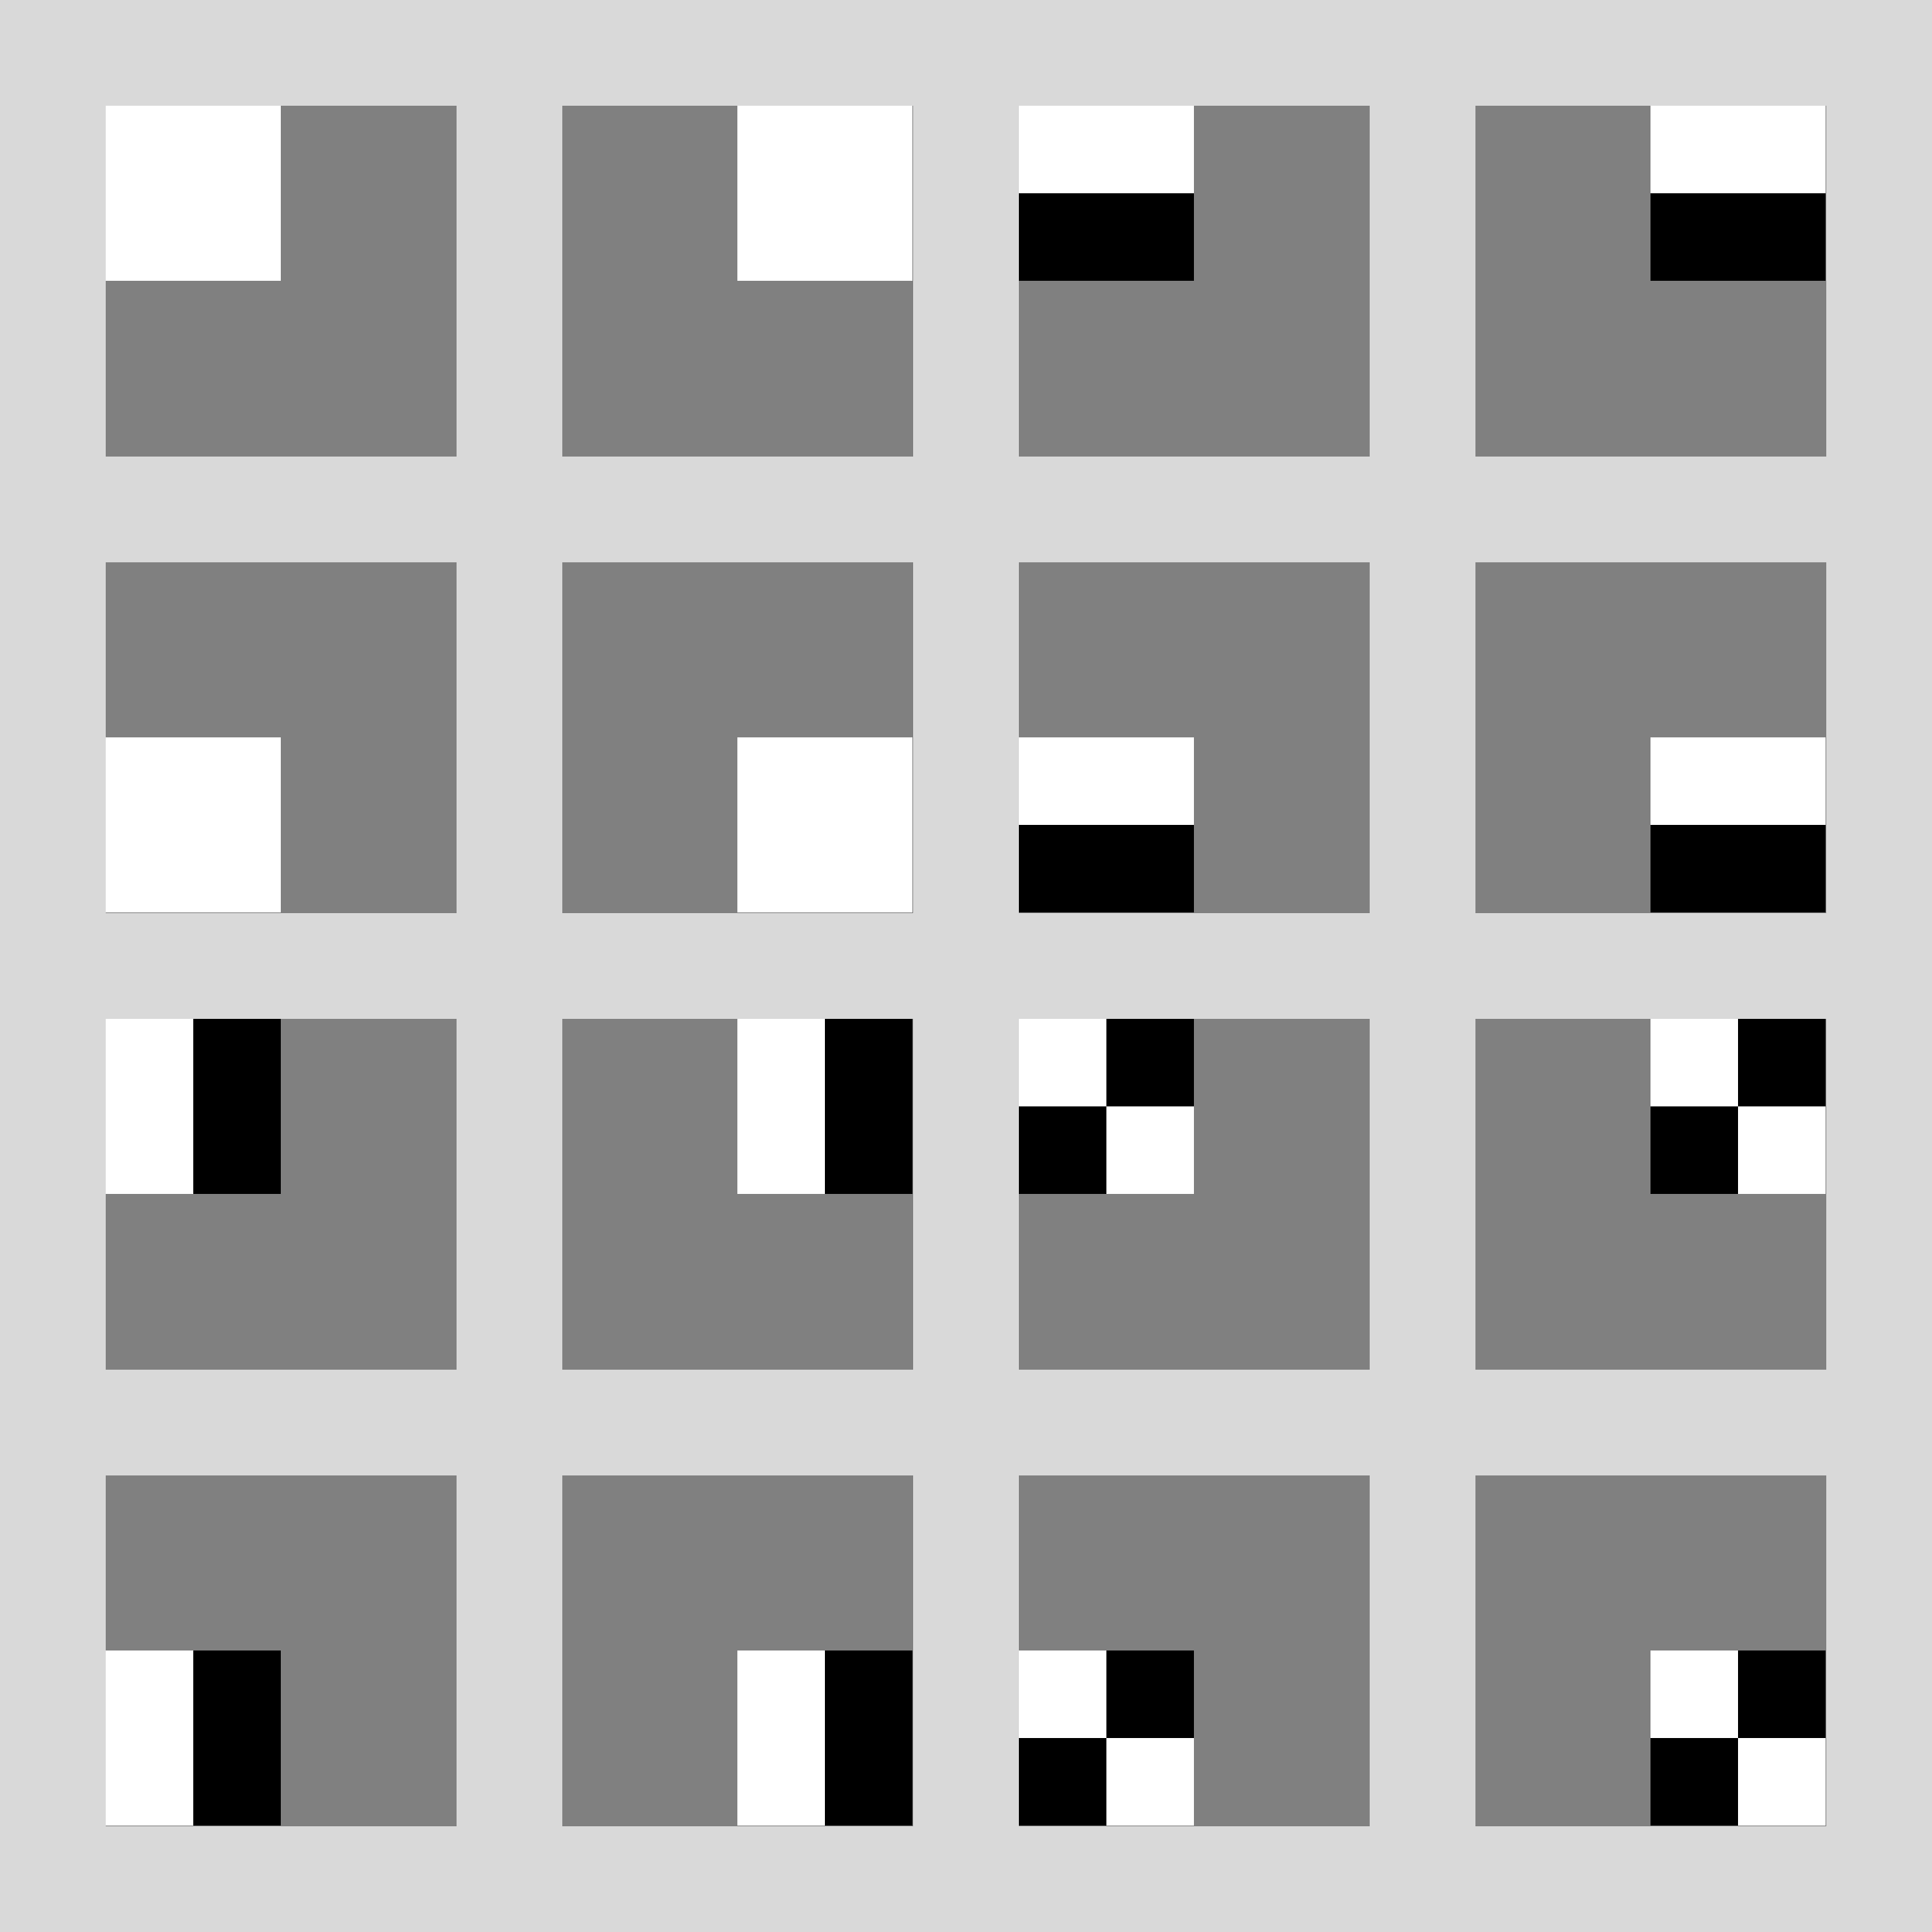
\includegraphics[width=\textwidth]{Chapter3/Images/haar2_scale1.png}
  \caption{Scale 1}
\end{subfigure}
\begin{subfigure}{0.4\textwidth}
  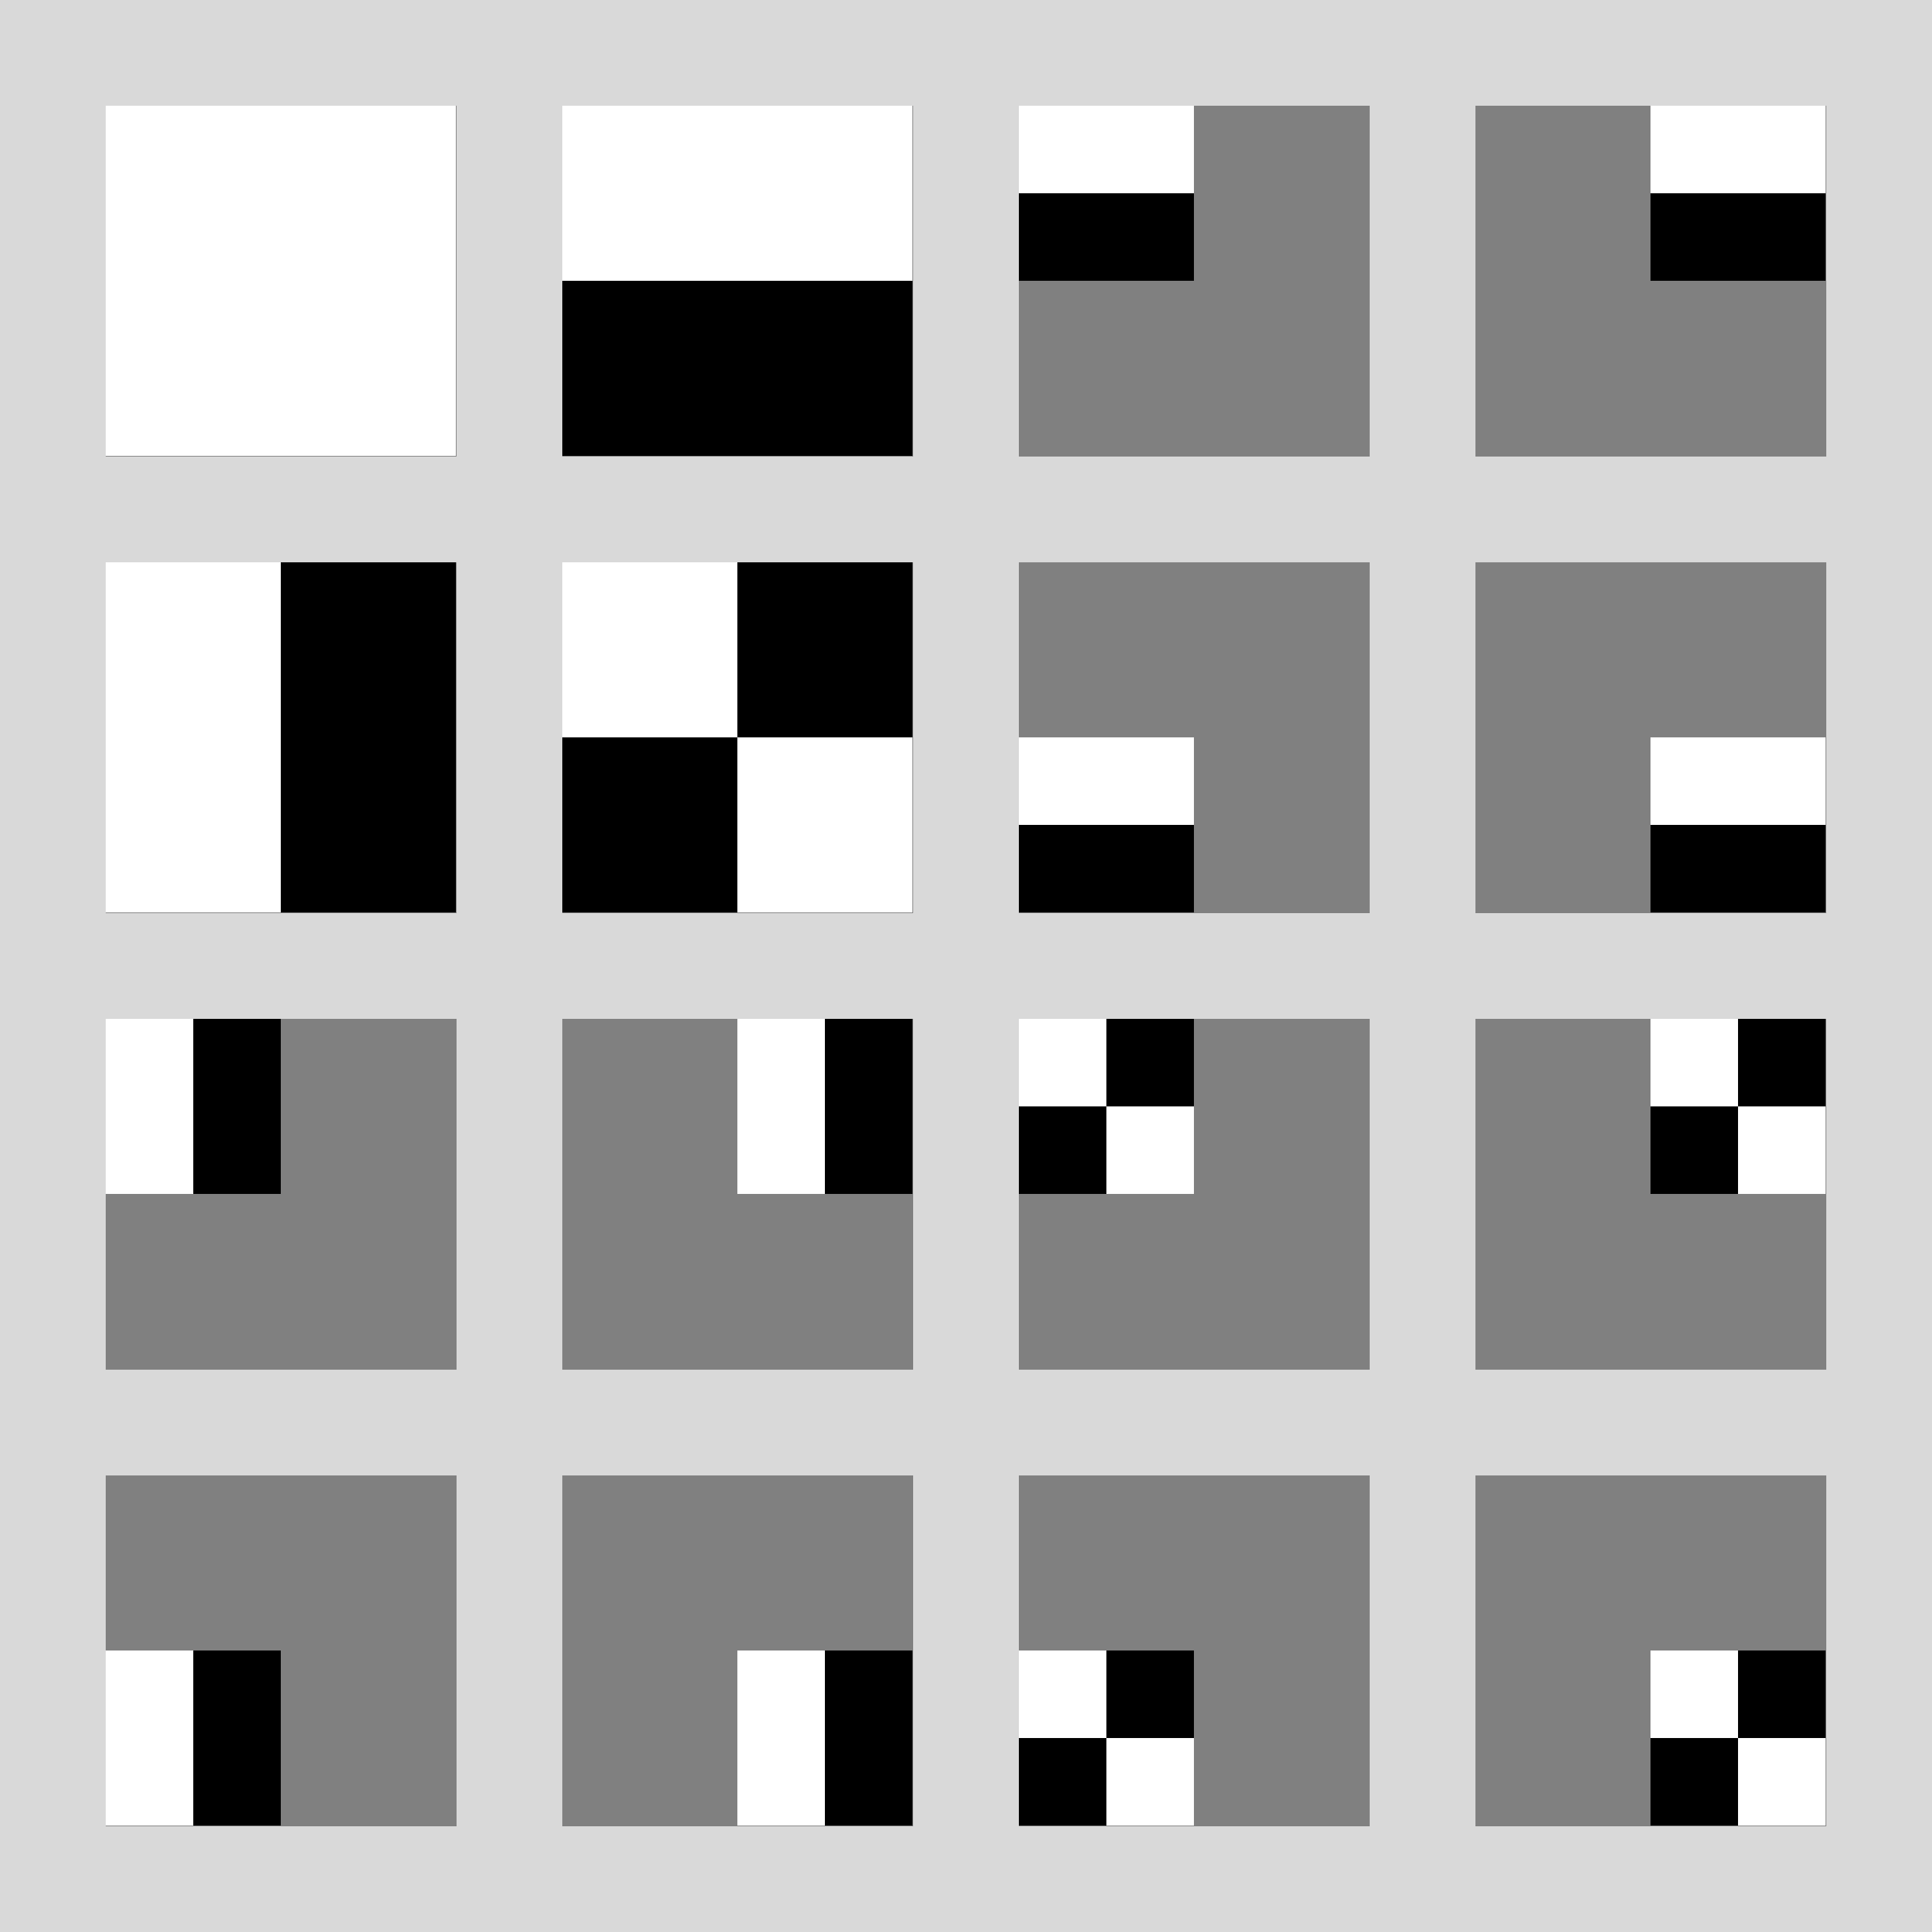
\includegraphics[width=\textwidth]{Chapter3/Images/haar2_scale2.png}
  \caption{Scale 2}
\end{subfigure}
\caption[2-D Haar basis functions]{The haar basis functions at the first scale (a) and the second scale (b). The DWT would use these basis functions to decompose a $4\times 4$ image.}
\label{fig:haar2_basis}
\end{figure}

\begin{figure}
\centering
\begin{subfigure}{0.4\textwidth}
  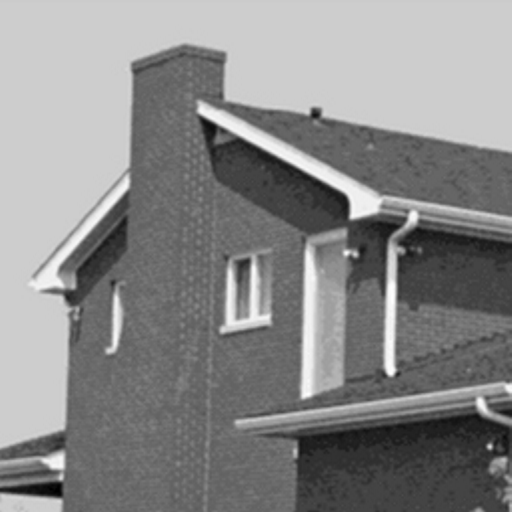
\includegraphics[width=\textwidth]{Chapter3/Images/house.png}
  \caption{Original $512\times 512$ image}
\end{subfigure}
\begin{subfigure}{0.4\textwidth}
  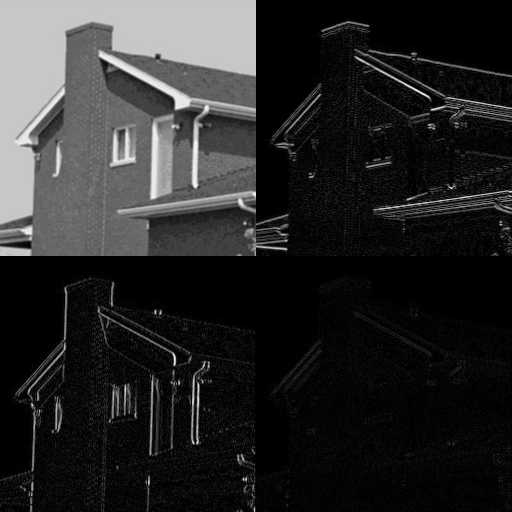
\includegraphics[width=\textwidth]{Chapter3/Images/dwt1.png}
  \caption{Scale 1 DWT}
\end{subfigure}
\begin{subfigure}{0.4\textwidth}
  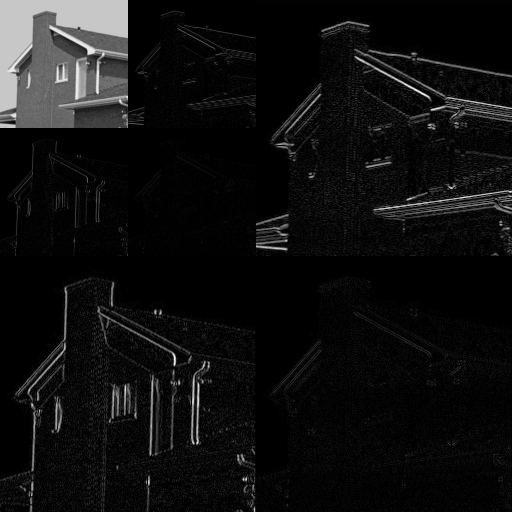
\includegraphics[width=\textwidth]{Chapter3/Images/dwt2.png}
  \caption{Scale 2 DWT}
\end{subfigure}
\begin{subfigure}{0.4\textwidth}
  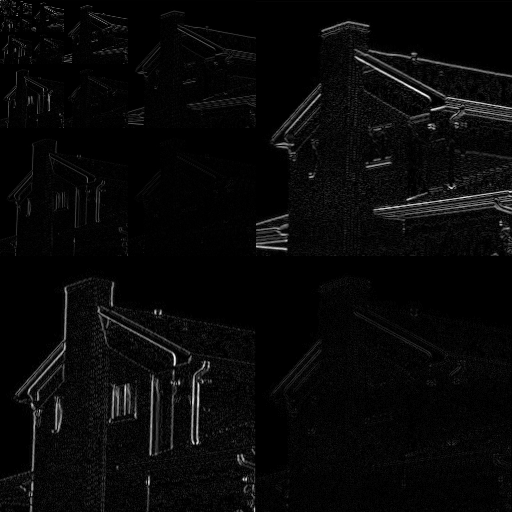
\includegraphics[width=\textwidth]{Chapter3/Images/dwt9.png}
  \caption{Scale 9 DWT}
\end{subfigure}
\caption[2-D Haar DWT Example]{The 2-D DWT using Haar wavelets of a digital image (a) of size $512\times 512$.
  We compute the DWT at the first and the second scale (b,c) as well as the full DWT (d).
  In (d), we have a single approximation coefficient at the top left corner.
  In (b,c,d), the brightness of a pixel increases monotonically with the size of the corresponding DWT coefficient.
  We have enhanced the detail coefficients (relative to the approximation coefficients) for better visibility.}
\label{fig:dwt2}
\end{figure}

% The wavelet basis functions for scale $j$ can be formed in two different ways.
% In the so-called ``standard'' construction \cite{stollnitz1995}, we first compute the DWT for scale $j$ for each column, followed by computing the scale-$J$ DWT on the intermediate result for each row.

The two-dimensional DWT of a signal is computed sequentially for each scale.
We start by computing the 1-D DWT at the first scale for each individual column.
Next, we do the same on each row of the intermediate result.
This gives us the 2-D DWT at the first scale.

To get the next highest scale, we perform the scale 1 computations on the approximation coefficients of the current scale.
This process process needs to be repeated $j$ times to obtain the DWT at $j$th scale.
\footnote{
  This construction procedure is the so-called ``non-standard'' construction.
  For an alternative construction strategy that leads to a different set of 2-D basis functions, see \cite{stollnitz1995}.
}

In Figure \ref{fig:haar2_basis}, we illustrate the basis functions resulting corresponding to the 2-D DWT with Haar wavelets..
We show two sets of basis functions that can be used to decompose a signal of size $4\times 4$, one corresponding to the first scale decomposition (panel (a)) and another set corresponding to the scale 2 (panel (b)).

In Figure \ref{fig:dwt2}, we have computed the DWT of a digital image at various scales. 
One can clearly see that the high-pass filters corresponding to the Haar wavelets act as edge detectors.


%\section{Three-Dimensional Basis Functions}
\subsection{Haar Wavelets for Videos}
A straightforward way of approaching the Discrete Wavelet Transform of a video would be to perform the two-dimensional DWT on each individual frame. 
This ``pseudo 3D'' approach is relatively simple, but typically also very inefficient.
We expect there to be continuity between successive frames of a video.
The pseudo 3D approach does not let us exploit any of the temporal correlations that are common in video signals.

A better approach would be to perform a full 3-D wavelet decomposition using three-dimensional scaling and wavelet functions.
In 3-D, we have one scaling function $\phi(x,y,t)$ and a total of $2^3-1=7$ wavelet functions.
These can be obtained by multiplying the 2-D functions in (\ref{eqn:2d_haar_wavelets}) with the scaling function $\phi(t)$ and the wavelet function $\psi(t)$ in the time domain:
\begin{equation*}
  \begin{split}
    \phi(x,y,t) &= \phi(t) \phi(x) \phi(y)\\
    \psi^H(x,y,t) &=\phi(t) \phi(x) \psi(y) \\
    \psi^V(x,y,t) &=\phi(t) \psi(x) \phi(y) \\
    \psi^D(x,y,t) &=\phi(t) \psi(x) \psi(y) \\
    \psi^T(x,y,t) &= \psi(t) \phi(x) \phi(y)\\
    \psi^{HT}(x,y,t) &=\psi(t) \phi(x) \psi(y) \\
    \psi^{VT}(x,y,t) &=\psi(t) \psi(x) \phi(y) \\
    \psi^{DT}(x,y,t) &=\psi(t) \psi(x) \psi(y)
  \end{split}
\end{equation*}
We use the $T$ superscript to denote the high-pass filters in the temporal direction.

\begin{figure}
\centering
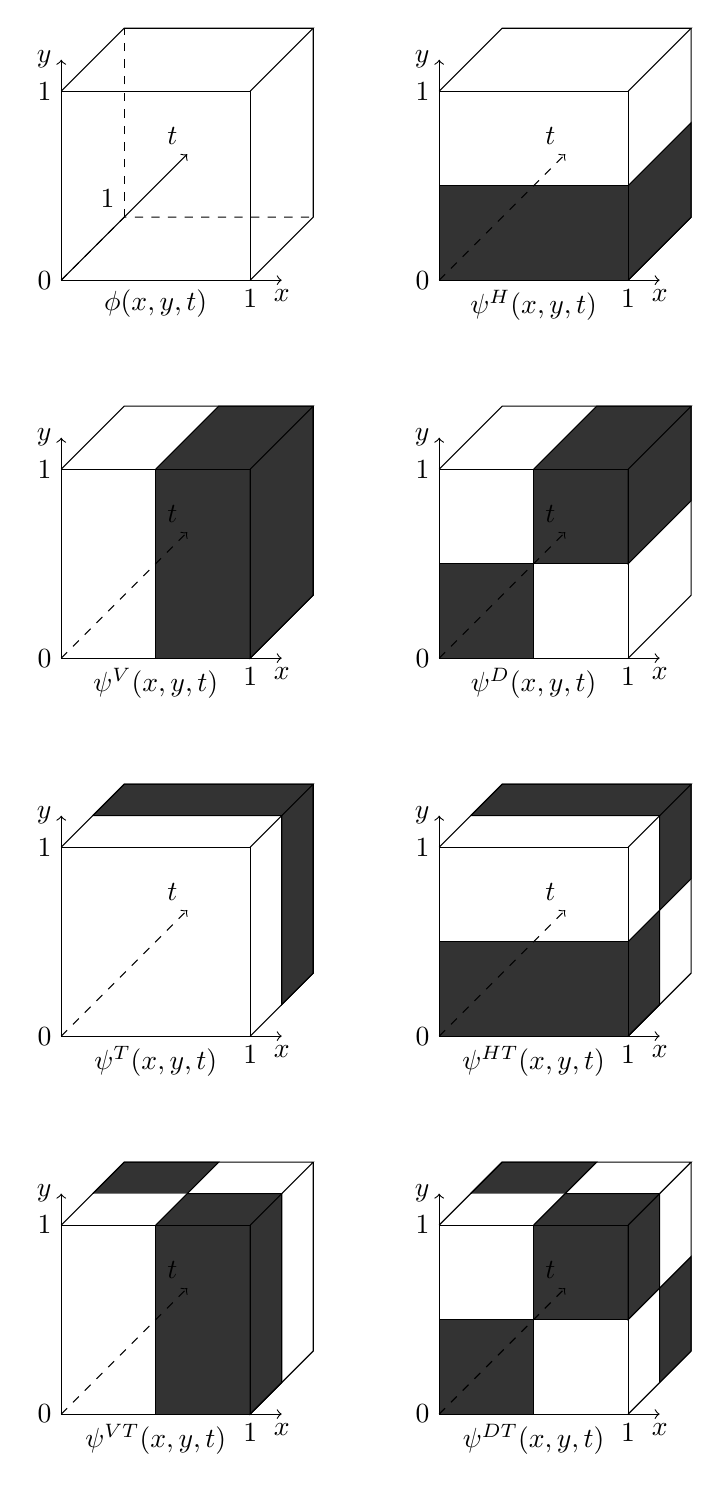
\begin{tikzpicture} [scale=0.8]
% top 4
  \draw [<->] (0,21.5) -- (0,18) -- (3.5,18);
  \draw [->] (0,18) -- (2,20);
  \draw (0,18) rectangle (3,21);
  \draw (0,21) -- (1,22) -- (4,22) -- (3,21);
  \draw (4,22) -- (4,19) -- (3,18);
  \draw [dashed] (0,18) -- (1,19) -- (4,19);
  \draw [dashed] (1,19) -- (1,22);

  \draw [<->] (6,21.5) -- (6,18) -- (9.5,18);
  \draw [->,dashed] (6,18) -- (8,20);
  \draw (6,18) rectangle (9,21);
  \draw (6,21) -- (7,22) -- (10,22) -- (9,21);
  \draw (10,22) -- (10,19) -- (9,18);

  \draw [<->] (0,15.5) -- (0,12) -- (3.5,12);
  \draw [->,dashed] (0,12) -- (2,14);
  \draw (0,12) rectangle (3,15);
  \draw (0,15) -- (1,16) -- (4,16) -- (3,15);
  \draw (4,16) -- (4,13) -- (3,12);

  \draw [<->] (6,15.5) -- (6,12) -- (9.5,12);
  \draw [->,dashed] (6,12) -- (8,14);
  \draw (6,12) rectangle (9,15);
  \draw (6,15) -- (7,16) -- (10,16) -- (9,15);
  \draw (10,16) -- (10,13) -- (9,12);
  
  \node at (1.5,18) [below] {$\phi(x,y,t)$};
  \node at (0,18) [left] {$0$};
  \node at (0,21) [left] {$1$};
  \node at (3,18) [below] {$1$};
  \node at (3.5,18) [below] {$x$};
  \node at (0,21.5) [left] {$y$};
  \node at (2,20) [above left] {$t$};
  \node at (1,19.3) [left] {$1$};
  
  \node at (7.5,18) [below] {$\psi^H(x,y,t)$};
  \node at (6,18) [left] {$0$};
  \node at (6,21) [left] {$1$};
  \node at (9,18) [below] {$1$};
  \node at (9.5,18) [below] {$x$};
  \node at (6,21.5) [left] {$y$};
  \node at (8,20) [above left] {$t$};

  \node at (1.5,12) [below] {$\psi^V(x,y,t)$};
  \node at (0,12) [left] {$0$};
  \node at (0,15) [left] {$1$};
  \node at (3,12) [below] {$1$};
  \node at (3.5,12) [below] {$x$};
  \node at (0,15.5) [left] {$y$};
  \node at (2,14) [above left] {$t$};

  \node at (7.5,12) [below] {$\psi^D(x,y,t)$};
  \node at (6,12) [left] {$0$};
  \node at (6,15) [left] {$1$};
  \node at (9,12) [below] {$1$};
  \node at (9.5,12) [below] {$x$};
  \node at (6,15.5) [left] {$y$};
  \node at (8,14) [above left] {$t$};

%bottom 4
  \draw [<->] (0,9.5) -- (0,6) -- (3.5,6);
  \draw [->,dashed] (0,6) -- (2,8);
  \draw (0,6) rectangle (3,9);
  \draw (0,9) -- (1,10) -- (4,10) -- (3,9);
  \draw (4,10) -- (4,7) -- (3,6);
  
  \draw [<->] (6,9.5) -- (6,6) -- (9.5,6);
  \draw [->,dashed] (6,6) -- (8,8);
  \draw (6,6) rectangle (9,9);
  \draw (6,9) -- (7,10) -- (10,10) -- (9,9);
  \draw (10,10) -- (10,7) -- (9,6);

  \draw [<->] (0,3.5) -- (0,0) -- (3.5,0);
  \draw [->,dashed] (0,0) -- (2,2);
  \draw (0,0) rectangle (3,3);
  \draw (0,3) -- (1,4) -- (4,4) -- (3,3);
  \draw (4,4) -- (4,1) -- (3,0);

  \draw [<->] (6,3.5) -- (6,0) -- (9.5,0);
  \draw [->,dashed] (6,0) -- (8,2);
  \draw (6,0) rectangle (9,3);
  \draw (6,3) -- (7,4) -- (10,4) -- (9,3);
  \draw (10,4) -- (10,1) -- (9,0);
  
  \node at (1.5,6) [below] {$\psi^T(x,y,t)$};
  \node at (0,6) [left] {$0$};
  \node at (0,9) [left] {$1$};
  \node at (3,6) [below] {$1$};
  \node at (3.5,6) [below] {$x$};
  \node at (0,9.5) [left] {$y$};
  \node at (2,8) [above left] {$t$};

  \node at (7.5,6) [below] {$\psi^{HT}(x,y,t)$};
  \node at (6,6) [left] {$0$};
  \node at (6,9) [left] {$1$};
  \node at (9,6) [below] {$1$};
  \node at (9.5,6) [below] {$x$};
  \node at (6,9.5) [left] {$y$};
  \node at (8,8) [above left] {$t$};

  \node at (1.5,0) [below] {$\psi^{VT}(x,y,t)$};
  \node at (0,0) [left] {$0$};
  \node at (0,3) [left] {$1$};
  \node at (3,0) [below] {$1$};
  \node at (3.5,0) [below] {$x$};
  \node at (0,3.5) [left] {$y$};
  \node at (2,2) [above left] {$t$};

  \node at (7.5,0) [below] {$\psi^{DT}(x,y,t)$};
  \node at (6,0) [left] {$0$};
  \node at (6,3) [left] {$1$};
  \node at (9,0) [below] {$1$};
  \node at (9.5,0) [below] {$x$};
  \node at (6,3.5) [left] {$y$};
  \node at (8,2) [above left] {$t$};
  % fills
  % top
  %TH
  \draw [fill=black, fill opacity=0.8] (6,18) rectangle (9,19.5);
  \draw [fill=black, fill opacity=0.8] (9,19.5) -- (10,20.5) -- (10,19) -- (9,18);
 
  % V
  \draw [fill=black, fill opacity=0.8] (1.5,12) rectangle (3,15);
  \draw [fill=black, fill opacity=0.8] (1.5,15) -- (2.5,16) -- (4,16) -- (4,13) -- (3,12) -- (3,15);

  %TD
  \draw [fill=black, fill opacity=0.8] (6,12) rectangle (7.5,13.5);
  \draw [fill=black, fill opacity=0.8] (7.5,13.5) rectangle (9,15);
  \draw [fill=black, fill opacity=0.8] (7.5,15) -- (8.5,16) -- (10,16) -- (10,14.5) -- (9,13.5) -- (9,15);
    
  % bottom
  % T
  \draw [fill=black, fill opacity=0.8] (0.5,9.5) -- (1,10) -- (4,10) -- (4,7) -- (3.5,6.5) -- (3.5,9.5) -- (0.5,9.5);
  %TH
  \draw [fill=black, fill opacity=0.8] (6,6) rectangle (9,7.5);
  \draw [fill=black, fill opacity=0.8] (6.5,9.5) -- (7,10) -- (10,10) -- (10,8.5) -- (9.5,8) -- (9.5,9.5) -- (6.5,9.5);
  \draw [fill=black, fill opacity=0.8] (9,7.5) -- (9.5,8) -- (9.5,6.5) -- (9,6);
  %TV
  \draw [fill=black, fill opacity=0.8] (1.5,0) rectangle (3,3);
  \draw [fill=black, fill opacity=0.8] (1.5,3) -- (2,3.5) -- (3.5,3.5) -- (3.5,0.5) -- (3,0) -- (3,3);
  \draw [fill=black, fill opacity=0.8] (0.5,3.5) -- (1,4) -- (2.5,4) -- (2,3.5);
  %TD
  \draw [fill=black, fill opacity=0.8] (6,0) rectangle (7.5,1.5);
  \draw [fill=black, fill opacity=0.8] (7.5,1.5) rectangle (9,3);
  \draw [fill=black, fill opacity=0.8] (7.5,3) -- (8,3.5) -- (9.5,3.5) -- (9.5,2) -- (9,1.5) -- (9,3);
  \draw [fill=black, fill opacity=0.8] (9.5,0.5) -- (9.5,2) -- (10,2.5) -- (10,1);
  \draw [fill=black, fill opacity=0.8] (6.5,3.5) -- (7,4) -- (8.5,4) -- (8,3.5);
\end{tikzpicture}
\caption[3-D Haar Wavelets]{The 3-D Haar scaling function and wavelet functions.
  Inside the $[0,1]\times [0,1] \times [0,1]$ cube, white corresponds to $+1$ and black corresponds to $-1$.
The functions are zero outside of the cube.}
\label{fig:haar_3d}
\end{figure}

\begin{figure}
  \centering
  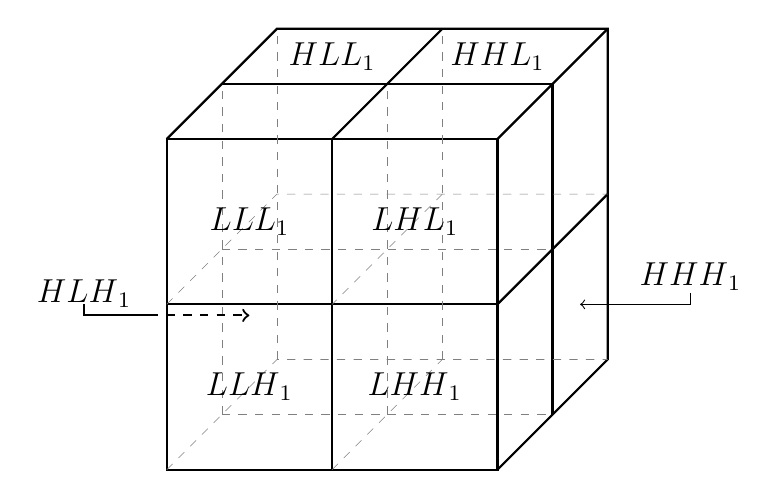
\begin{tikzpicture}[scale = 0.7]
    \draw [thick] (0,0) rectangle (6,6);
    \draw [thick] (0,3) -- (6,3);
    \draw [thick] (3,0) -- (3,6);
    \draw [thick] (0,6) -- (2,8) -- (8,8) -- (8,2) -- (6,0);
    \draw [thick] (1,7) -- (7,7) -- (7,1);
    \draw [thick] (6,6) -- (8,8);
    \draw [thick] (6,3) -- (8,5);
    \draw [thick] (3,6) -- (5,8);
    \draw [dashed,gray,very thin] (0,0) -- (2,2) -- (8,2);
    \draw [dashed,gray,very thin] (2,2) -- (2,8);
    \draw [dashed,gray,very thin] (1,1) -- (7,1);
    \draw [dashed,gray,very thin] (0,3) -- (2,5) -- (8,5);
    \draw [dashed,gray,very thin] (5,5) -- (3,3);
    \draw [dashed,gray,very thin] (1,4) -- (7,4);
    \draw [dashed,gray,very thin] (3,0) -- (5,2);
    \draw [dashed,gray,very thin] (4,1) -- (4,7);
    \draw [dashed,gray,very thin] (5,2) -- (5,8);
    \draw [dashed,gray,very thin] (1,1) -- (1,7);
    \node at (6,7.5) {\large$\bm{HHL}_1$};
    \node at (3,7.5) {\large$\bm{HLL}_1$};
    \node at (1.5,4.5) {\large$\bm{LLL}_1$};
    \node at (4.5,4.5) {\large$\bm{LHL}_1$};
    \node at (1.5,1.5) {\large$\bm{LLH}_1$};
    \node at (4.5,1.5) {\large$\bm{LHH}_1$};
    \node at (9.5,3.5) {\large$\bm{HHH}_1$};
    \draw [<-] (7.5,3) -- (9.5,3) -- (9.5,3.2);
    \node at (-1.5,3.2) {\large$\bm{HLH}_1$};
    \draw [thick](-1.5,3) -- (-1.5,2.8) -- (-0.3,2.8);
    \draw [->,dashed,thick] (-0.3,2.8) -- (1.5,2.8);
  \end{tikzpicture}
  \caption[Wavelet decomposition of a video]{The wavelet decomposition of a three-dimensional signal $v(x,y,t)$ at the first scale. 
    $L$ stands for ``low'' and $H$ stands for ``high''.
    To obtain the decomposition at higher scales, we recursively decompose the low-pass channels $\bm{LLL}_j$ in a similar way.}
  \label{fig:3d_channels}
\end{figure}

\begin{figure}
\centering
  \begin{subfigure}{0.35\textwidth}
    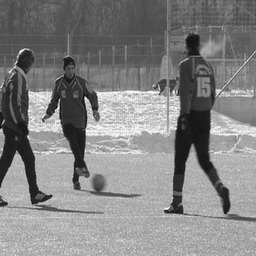
\includegraphics[width=0.9\textwidth]{Chapter3/Images/frame_11.png}
    \caption{Frame 11}
  \end{subfigure}
  \begin{subfigure}{0.35\textwidth}
    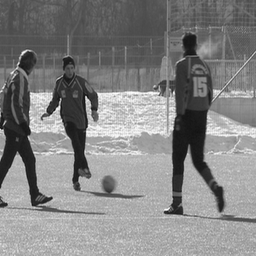
\includegraphics[width=0.9\textwidth]{Chapter3/Images/frame_12.png}
    \caption{Frame 12}
  \end{subfigure}
  \begin{subfigure}{0.35\textwidth}
    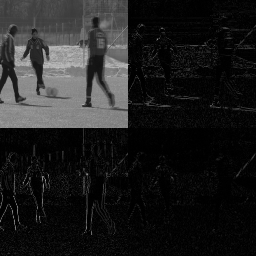
\includegraphics[width=0.9\textwidth]{Chapter3/Images/dwt_6.png}
    \caption{Scale 1 DWT: ``frame'' 6}
  \end{subfigure}
  \begin{subfigure}{0.35\textwidth}
    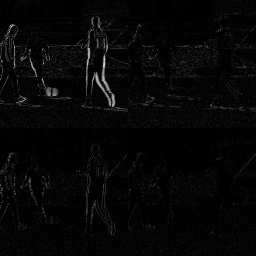
\includegraphics[width=0.9\textwidth]{Chapter3/Images/dwt_38.png}
    \caption{Scale 1 DWT: ``frame'' 38}
  \end{subfigure}
  \caption[Example showing the Haar wavelet decomposition of a video signal]{Frames 11 and 12 of a 64-frame video with a resolution of $256\times 256$ (a,b).
    We perform the three-dimensional DWT at the first scale using Haar wavelets and show two ``slices'' of the resulting coefficients (c,d). The detail coefficients have been enhanced to improve visibility.}
 \label{fig:3d_dwt}
\end{figure}

Figure \ref{fig:haar_3d} shows the 3-D scaling and wavelet functions for the Haar wavelets.
To obtain the basis functions corresponding to the 3-D Haar wavelet domain, we compute scaled and shifted versions of these functions:% (\ref{eqn:haar_scaling_basis}) and (\ref{eqn:haar_wavelet_basis}).
\begin{equation*}
  \phi_{k_1,k_2,k_3}^j(x,y,t) = 2^{3j/2} \phi(2^j t - k_3)\phi(2^j x - k_1) \phi(2^j y - k_2)
\end{equation*}

At the first scale, the 3-D wavelet decomposition of a video results in 8 distinct channels: one corresponding to a low-pass filter, and 7 corresponding to high-pass filters in various directions.
The approximation and detail coefficients of the various filters will be arranged as in Figure \ref{fig:3d_channels}.

For the Haar wavelets, the high-pass filters act as edge detectors, just like in the 2-D case. 
However, on top of detecting edges along spatial directions, we also get high-pass filters that detect sudden changes in the temporal direction, i.e. motion detectors.

As an example, consider Figure \ref{fig:3d_dwt}.
In panels (a) and (b), we show two adjacent frames of the ``soccer'' test video.
We perform the 3-D DWT using Haar basis functions at the first scale.
At scale one, the 3-D Haar basis functions have support over a $2\times 2\times 2$ volume.
Thus, all the DWT coefficients that are affected by the data in frames 11 and 12 of the original video, are contained within two ``frames'', or ``slices'', of the transformed signal.
For frames 11 and 12 of the original 64-frame video, these slices are at positions $12/2=6$ and $(6+64)/2=38$ in the transformed video.

In panel (c), we see the spatial edge detectors (the $LLH$, $LHL$ and $LHH$ channels) that are similar to those in the 2-D case (Figure \ref{fig:dwt2}).
The top left corner corresponds to the low-pass filter $LLL$ and can be regarded as an ``average'' of the video.

Panel (d), shows the four channels associated with a high-pass filter in the temporal direction.
The $HLL$ channel (top left corner of panel (d)) picks up overall differences in adjacent frames.
In this example, we note that it detects the motion of the football players and the ball, (as well as a slight motion of the background due to the panning of the camera).
The remaining channels in panel (d) combine motion detection with edge detection.






\section{Construction of the Basis Matrix \texorpdfstring{$\bm\Psi$}{[Psi]}}
So far, when discussing basis transforms in two or three dimensions, we regarded the signal $\bm v$ as a 2-D or 3-D array, respectively.
However, the theory in Chapter \ref{ch:cs} was developed for signals in vectorized forms.
Moreover, in Chapter \ref{ch:rvm} we will discuss the RVM which also operates on vectorized data.
Therefore, it is important that we discuss how to vectorize our multi-dimensional signals.

In this section we will define the vectorization scheme that we used in our implementation and describe how to construct the basis matrix $\bm\Psi$ from the respective transform matrices in a way that is consistent with the vectorization.

\subsection{Basis Matrix for One-Dimensional Signals}
We start with 1-D signals. 
This case is trivial, since a one-dimensional signal $\bm v$ can directly be treated as a vector in $\mathbb{R}^M$, where $M$ is the length of the signal.

The basis matrix matrix, in this case, is simply the inverse transform matrix.
So, for the DCT, the basis matrix is $\bm\Psi = \bm P$, where $\bm P$ is defined in equation (\ref{eqn:idct_basis}).
We have defined the basis matrix corresponding to the discrete Haar wavelet transform in equation (\ref{eqn:haar1_basis}).

\subsection{Basis Matrix for Two-Dimensional Signals}
\label{sect:vectorize2d}
Suppose $\bm A$ is a two-dimensional signal of size $r\times c$ (i.e. $r$ rows and $c$ columns).
Suppose further that $r$ and $c$ are powers of 2, $r=2^{q_1}$ and $c = 2^{q_2}$, say.

We vectorize $\bm A$ in a row-major fashion.
To be explicit, let $\bm a_j^T$ be the $j$th row of $\bm A\in\mathbb{R}^{r\times c}$.
The vectorized form of $\bm A$ is then given by
\begin{equation*}
  \bm v = \begin{bmatrix}
    \bm a_1 \\
    \bm a_2 \\
    \vdots \\
    \bm a_r
  \end{bmatrix}
\end{equation*}
Thus, we end up with a long vector $\bm v \in \mathbb{R}^{rc}$.

\subsubsection{DCT}
To form the basis matrix corresponding to the two-dimensional DCT, we use the DCT's seperability property.
Let $\bm\Psi_r$ and $\bm\Psi_c$ be the DCT basis matrices corresponding to one-dimensional signals of length $r$ and $c$, respectively.
The basis matrix corresponding to $\bm v$ is then constructed by forming the \emph{kronecker product} of $\bm\Psi_c$ and $\bm\Psi_r$:
\begin{equation*}
\label{eqn:dct3_basis}
  \bm\Psi = \bm\Psi_c \otimes \bm\Psi_r
\end{equation*}

The kronecker product $P \otimes Q$ between matrices $P$ and $Q$ with dimensions $m_P \times n_P$ and $m_Q \times n_Q$, respectively,  is defined by the block matrix
\begin{equation}
\label{eqn:kron}
\begin{bmatrix}
P_{1,1} Q & P_{1,2} Q & \cdots & P_{1,n_P} Q \\
P_{2,1} Q & P_{2,2} Q & \cdots & P_{2,n_P} Q \\
\vdots&\vdots&\ddots&\vdots \\
P_{m_P,1} Q & P_{m_P,2} Q & \cdots & P_{m_P,n_P} Q \\
\end{bmatrix}
\end{equation}
of size $(m_Pm_Q) \times (n_Pn_Q)$.

\subsubsection{DWT}
For the 2-D Haar DWT at the first scale, the basis matrix is constructed in a similar fashion.
Let $\bm H^{q_1}$ and $\bm H^{q_2}$ be defined according to equation (\ref{eqn:haar_H}), and let $\bm G^{q_1}$ and $\bm G^{q_2}$  be formed according to (\ref{eqn:haar_G}) (where we dropped the $haar$ subscript). 
The basis matrix $\bm\Psi$ is constructed as follows:
\begin{equation*}
%  \resizebox{.9\hsize}{!}{$ 
 \bm \Psi = 
  \begin{bmatrix}
    \bm H^{q_2} \otimes\bm H^{q_1} \\
    \bm H^{q_2} \otimes \bm G^{q_1} \\
    \bm G^{q_2} \otimes \bm H^{q_1} \\
    \bm G^{q_2} \otimes \bm G^{q_1} 
  \end{bmatrix}^T.
%$}
\end{equation*}
For a signal of size $2^{q_1}\times 2^{q_2}$, we can build a cascade up to the $q$th scale, where $q = \min\{q_1,q_2\}$.
The resulting basis matrix is given by
\begin{equation*}
\label{eqn:haar2_fullbasis}
%  \resizebox{.9\hsize}{!}{$
  \bm \Psi = 
  \begin{bmatrix}
    (\bm H^{q_2-q}\bm H^{q_2-q+1} \cdots \bm H^{q_2}) \otimes (\bm H^{q_1-q} \bm H^{q_1-q+1}\cdots\bm H^{q_1}) \\
    (\bm H^{q_2-q}\bm H^{q_2-q+1} \cdots \bm H^{q_2}) \otimes (\bm G^{q_1-q} \bm H^{q_1-q+1}\cdots\bm H^{q_1}) \\
    (\bm G^{q_2-q}\bm H^{q_2-q+1} \cdots \bm H^{q_2}) \otimes (\bm H^{q_1-q} \bm H^{q_1-q+1}\cdots\bm H^{q_1}) \\
    (\bm G^{q_2-q}\bm H^{q_2-q+1} \cdots \bm H^{q_2}) \otimes (\bm G^{q_1-q} \bm H^{q_1-q+1}\cdots\bm H^{q_1}) \\
    (\bm H^{q_2-q+1}\bm H^{q_2-q+2} \cdots \bm H^{q_2}) \otimes (\bm G^{q_1-q+1} \bm H^{q_1-q+2}\cdots\bm H^{q_1}) \\
    (\bm G^{q_2-q+1}\bm H^{q_2-q+2} \cdots \bm H^{q_2}) \otimes (\bm H^{q_1-q+1} \bm H^{q_1-q+2}\cdots\bm H^{q_1}) \\
    (\bm G^{q_2-q+1}\bm H^{q_2-q+2} \cdots \bm H^{q_2}) \otimes (\bm G^{q_1-q+1} \bm H^{q_1-q+2}\cdots\bm H^{q_1}) \\
    \vdots \\
    (\bm G^{q_2-2}\bm H^{q_2-1} \bm H^{q_2}) \otimes (\bm G^{q_1-2}\bm H^{q_1-1}\bm H^{q_1}) \\
    (\bm H^{q_2-1} \bm H^{q_2}) \otimes (\bm G^{q_1-1}\bm H^{q_1}) \\
    (\bm G^{q_2-1} \bm H^{q_2}) \otimes (\bm H^{q_1-1}\bm H^{q_1}) \\
    (\bm G^{q_2-1} \bm H^{q_2}) \otimes (\bm G^{q_1-1}\bm H^{q_1}) \\
    \bm H^{q_2} \otimes \bm G^{q_1} \\
    \bm G^{q_2} \otimes \bm H^{q_1} \\
    \bm G^{q_2} \otimes \bm G^{q_1} 
  \end{bmatrix}^T.
%$}
\end{equation*}
Note that the dimensions of the basis matrix are $(rc)\times (rc)$, regardless of the scale that we use.

\subsection{Basis Matrix for Three-Dimensional Signals}

Let $\bm V$ be a video signal of size $r\times c\times f$ ($r$ rows, $c$ columns and $f$ frames), where $r=2^{q_1}$, $c=2^{q_2}$ and $f=2^{q_3}$.

We vectorize $\bm V$ by first vectorizing each individual frame in a row-major fashion (as in the 2-D case), followed by stacking the vectorized frames on top of each other.
The result $\bm v$ is a long vector of length $rcf$.

\subsubsection{DCT}
The basis matrix corresponding to the DCT is given by 
\begin{equation*}
  \bm\Psi = \bm\Psi_f\otimes\bm\Psi_c\otimes\bm\Psi_r
\end{equation*}
where $\bm\Psi_r$, $\bm\Psi_c$ and $\bm\Psi_f$ are the DCT basis matrices for 1-D signals (\ref{eqn:idct_basis}) of length $r$, $c$ and $f$, respectively.

\subsubsection{Haar}
The Haar basis matrix for video signals at scale 1 is constructed as follows:
\begin{equation*}
  \bm\Psi = 
  \begin{bmatrix}
    \bm H^{q_3}\otimes \bm H^{q_2} \otimes\bm H^{q_1} \\
    \bm H^{q_3}\otimes \bm H^{q_2} \otimes \bm G^{q_1} \\
    \bm H^{q_3}\otimes \bm G^{q_2} \otimes \bm H^{q_1} \\
    \bm H^{q_3}\otimes \bm G^{q_2} \otimes \bm G^{q_1} \\
    \bm G^{q_3}\otimes \bm H^{q_2} \otimes\bm H^{q_1} \\
    \bm G^{q_3}\otimes \bm H^{q_2} \otimes \bm G^{q_1} \\
    \bm G^{q_3}\otimes \bm G^{q_2} \otimes \bm H^{q_1} \\
    \bm G^{q_3}\otimes \bm G^{q_2} \otimes \bm G^{q_1} 
  \end{bmatrix}^T.
\end{equation*}
where the matrices $\bm H$ and $\bm G$ are defined in equations (\ref{eqn:haar_H}) and (\ref{eqn:haar_G}).

The extension to higher scales is similar to equation (\ref{eqn:haar2_fullbasis}).
We can build the matrix up until the $q$th scale, where $q=\min\{q_1,q_2,q_3\}$.
The full basis matrix is
\begin{equation*}
  \resizebox{.9\hsize}{!}{$
  \bm\Psi = 
  \begin{bmatrix}
    (\bm H^{q_3-q}\bm H^{q_3-q+1}\cdots\bm H^{q_3})\otimes (\bm H^{q_2-q}\bm H^{q_2-q+1}\cdots\bm H^{q_2}) \otimes (\bm H^{q_1-q}\bm H^{q_1-q+1}\cdots\bm H^{q_1}) \\
    (\bm H^{q_3-q}\bm H^{q_3-q+1}\cdots\bm H^{q_3})\otimes (\bm H^{q_2-q}\bm H^{q_2-q+1}\cdots\bm H^{q_2}) \otimes (\bm G^{q_1-q}\bm H^{q_1-q+1}\cdots\bm H^{q_1}) \\
    (\bm H^{q_3-q}\bm H^{q_3-q+1}\cdots\bm H^{q_3})\otimes (\bm G^{q_2-q}\bm H^{q_2-q+1}\cdots\bm H^{q_2}) \otimes (\bm H^{q_1-q}\bm H^{q_1-q+1}\cdots\bm H^{q_1}) \\
    (\bm H^{q_3-q}\bm H^{q_3-q+1}\cdots\bm H^{q_3})\otimes (\bm G^{q_2-q}\bm H^{q_2-q+1}\cdots\bm H^{q_2}) \otimes (\bm G^{q_1-q}\bm H^{q_1-q+1}\cdots\bm H^{q_1}) \\
    (\bm G^{q_3-q}\bm H^{q_3-q+1}\cdots\bm H^{q_3})\otimes (\bm H^{q_2-q}\bm H^{q_2-q+1}\cdots\bm H^{q_2}) \otimes (\bm H^{q_1-q}\bm H^{q_1-q+1}\cdots\bm H^{q_1}) \\
    (\bm G^{q_3-q}\bm H^{q_3-q+1}\cdots\bm H^{q_3})\otimes (\bm H^{q_2-q}\bm H^{q_2-q+1}\cdots\bm H^{q_2}) \otimes (\bm G^{q_1-q}\bm H^{q_1-q+1}\cdots\bm H^{q_1}) \\
    (\bm G^{q_3-q}\bm H^{q_3-q+1}\cdots\bm H^{q_3})\otimes (\bm G^{q_2-q}\bm H^{q_2-q+1}\cdots\bm H^{q_2}) \otimes (\bm H^{q_1-q}\bm H^{q_1-q+1}\cdots\bm H^{q_1}) \\
    (\bm G^{q_3-q}\bm H^{q_3-q+1}\cdots\bm H^{q_3})\otimes (\bm G^{q_2-q}\bm H^{q_2-q+1}\cdots\bm H^{q_2}) \otimes (\bm G^{q_1-q}\bm H^{q_1-q+1}\cdots\bm H^{q_1}) \\
    (\bm H^{q_3-q+1}\bm H^{q_3-q+2}\cdots\bm H^{q_3})\otimes (\bm H^{q_2-q+1}\bm H^{q_2-q+2}\cdots\bm H^{q_2}) \otimes (\bm G^{q_1-q+1}\bm H^{q_1-q+2}\cdots\bm H^{q_1}) \\
    (\bm H^{q_3-q+1}\bm H^{q_3-q+2}\cdots\bm H^{q_3})\otimes (\bm G^{q_2-q+1}\bm H^{q_2-q+2}\cdots\bm H^{q_2}) \otimes (\bm H^{q_1-q+1}\bm H^{q_1-q+2}\cdots\bm H^{q_1}) \\
    \vdots\\
    (\bm G^{q_3-1}\bm H^{q_3})\otimes (\bm G^{q_2-1}\bm H^{q_2}) \otimes (\bm G^{q_1-1}\bm H^{q_1}) \\
    \bm H^{q_3}\otimes \bm H^{q_2} \otimes \bm G^{q_1} \\
    \bm H^{q_3}\otimes \bm G^{q_2} \otimes \bm H^{q_1} \\
    \bm H^{q_3}\otimes \bm G^{q_2} \otimes \bm G^{q_1} \\
    \bm G^{q_3}\otimes \bm H^{q_2} \otimes \bm H^{q_1} \\
    \bm G^{q_3}\otimes \bm H^{q_2} \otimes \bm G^{q_1} \\
    \bm G^{q_3}\otimes \bm G^{q_2} \otimes \bm H^{q_1} \\
    \bm G^{q_3}\otimes \bm G^{q_2} \otimes \bm G^{q_1} 
  \end{bmatrix}^T
$}
\end{equation*}

For video signals, the basis matrix $\bm\Psi$ has dimensions $(hwf)\times(hwf)$.

